% vim: set textwidth=78 autoindent:

% \section{GRASS GIS Integration}\label{sec:grass}\index{GRASS}
\section{Intégration du SIG GRASS}\label{sec:grass}\index{GRASS}

% when the revision of a section has been finalized, 
% comment out the following line:
%\updatedisclaimer

%The GRASS plugin provides access to GRASS GIS~\cite{GRASSweb} databases and functionalities. This includes visualization of GRASS raster and vector 
%layers, digitizing vector layers, editing vector attributes, creating new vector layers and analysing GRASS 2D and 3D data with more than 300 GRASS 
%modules.
L'extension GRASS fourni un accès aux bases de données et aux fonctionnalités de GRASS. Cela inclut la visualisation des couches d'informations GRASS raster et vecteur, la numérisation de couches vecteurs, l'édition des attributs des couches d'informations vecteurs, la création de nouvelles couches et l'analyse 2D et 3D grâce à l'accès à près de 300 modules GRASS

%In this Section we'll introduce the plugin functionalities and give some examples on managing and working with GRASS data. Following main features 
%are provided with the toolbar menu, when you start the GRASS plugin, as described in Section~\ref{sec:starting_grass}:
Dans cette section, nous présenterons les fonctionnalités de l'extension et nous donnerons des exemples sur la manière de gérer et de travailler avec des données GRASS. Les fonctionnalités principales suivantes sont fournies dans la barre de menu lorsque vous lancez l'extension GRASS, comme décrit dans la section ~\ref{sec:starting_grass}:
\begin{itemize}
%\item \toolbtntwo{grass_open_mapset}{Open mapset}
%\item \toolbtntwo{grass_new_mapset}{New mapset}
%\item \toolbtntwo{grass_close_mapset}{Close mapset}
%\item \toolbtntwo{grass_add_vector}{Add GRASS vector layer}
%\item \toolbtntwo{grass_add_raster}{Add GRASS raster layer}
%\item \toolbtntwo{grass_new_vector_layer}{Create new GRASS vector}
%\item \toolbtntwo{grass_edit}{Edit GRASS vector layer}
%\item \toolbtntwo{grass_tools}{Open GRASS tools}
%%\item \toolbtntwo{grass_shell}{Open GRASS Shell}
%\item \toolbtntwo{grass_region}{Display current GRASS region} 
%\item \toolbtntwo{grass_region_edit}{Edit current GRASS region}
\item \toolbtntwo{grass_open_mapset}{Ouvrir le jeu de données}
\item \toolbtntwo{grass_new_mapset}{Nouveau jeu de données}
\item \toolbtntwo{grass_close_mapset}{Fermer le jeu de données}
\item \toolbtntwo{grass_add_vector}{Ajouter une couche vectorielle GRASS}
\item \toolbtntwo{grass_add_raster}{Ajouter une couche raster GRASS}
\item \toolbtntwo{grass_new_vector_layer}{Créer une nouvelle couche vectorielle GRASS}
\item \toolbtntwo{grass_edit}{Éditer une couche vectorielle GRASS}
\item \toolbtntwo{grass_tools}{Ouvrir les outils GRASS}
\item \toolbtntwo{grass_shell}{Ouvrir le shell GRASS}
\item \toolbtntwo{grass_region}{Afficher la région courante GRASS} 
\item \toolbtntwo{grass_region_edit}{Éditer la région courante GRASS}\end{itemize}

%\subsection{Starting the GRASS plugin}\label{sec:starting_grass}
\subsection{Lancer l'extension GRASS}\label{sec:starting_grass}\index{GRASS!Démarrage de QGIS} 

%To use GRASS functionalities and/or visualize GRASS vector and raster layers in QGIS, you must select and load the GRASS plugin with the Plugin Manager. 
%Therefore click the menu \mainmenuopt{Plugins} > \mainmenuopt{Manage Plugins},select \dropmenuopt{GRASS} and click \button{OK}. 

Pour pouvoir utiliser les fonctionnalités de GRASS et/ou visualiser des données vecteurs ou raster dans QGIS, vous devez sélectionner et charger l'extension GRASS à l'aide 
du gestionnaire d'extensions. Pour le faire cliquez sur le menu \mainmenuopt{Plugins} > \mainmenuopt{Gestionnaire de Plugins}, sélectionnez \dropmenuopt{GRASS} et cliquez sur \button{OK}. 


%You can now start loading raster and vector layers from an existing GRASS \filename{LOCATION} (see Section \ref{sec:load_grassdata}). Or you create a 
%new GRASS \filename{LOCATION} with QGIS (see Section \ref{sec:create_loc}) and import some raster and vector data (see Section \ref{sec:import_loc_data}) 
%for further analysis with the GRASS Toolbox (see Section 
Vous pouvez maintenant charger des données raster et vecteur depuis un \filename{SECTEUR} GRASS existant (voir Section \ref{sec:load_grassdata}). Ou alors vous pouvez créer un nouveau \filename{SECTEUR} GRASS à l'aide de QGIS (voir Section \ref{sec:create_loc}) et y importer des données raster et vecteur (voir Section \ref{sec:import_loc_data}) pour réaliser des traitements à l'aide de la boîte à outils GRASS.\ref{subsec:grass_toolbox}).


%\subsection{Loading GRASS raster and vector layers}\label{sec:load_grassdata}\index{GRASS!loading data}
\subsection{Charger des données GRASS raster et vecteur}\label{sec:load_grassdata}\index{GRASS!Chargement de données} 

%With the GRASS plugin, you can load vector or raster layers using the appropriate button on the toolbar menu. As an example we use the QGIS alaska
%dataset (see Section \ref{label_sampledata}). It includes a small sample GRASS \filename{LOCATION} with 3 vector layers and 1 raster elevation map.

Avec l'extension GRASS, vous pouvez charger des données raster ou vecteur l'aide du bouton approprié dans la barre de menu. Ici nous utiliserons comme exemple, le jeu de données QGIS Alaska (voir Section \ref{label_sampledata}). Il contient un \filename{SECTEUR} GRASS avec 3 couches vecteurs et 1 raster d'élévation.

\begin{enumerate}
  %\item Create a new folder \filename{grassdata}, download the QGIS alaska dataset \filename{qgis\_sample\_data.zip} from
  %\url{http://download.osgeo.org/qgis/data/} and unzip the file into
  %\filename{grassdata}. 
  \item Créez un nouveau répertoire \filename{grassdata}, téléchargez le jeu de données QGIS alaska \filename{qgis\_sample\_data.zip} depuis  \url{http://download.osgeo.org/qgis/data/} et décompressez le dans le répertoire \filename{grassdata}
  %\item Start QGIS.
  \item Démarrez QGIS
  %\item If not already done in a previous QGIS session, load the GRASS plugin clicking on \mainmenuopt{Plugins} > \mainmenuopt{Manage Plugins} and selecting \dropmenuopt{GRASS}. The GRASS toolbar appears on the toolbar menu.
  \item Si cela n'a pas déjà été fait dans une précédente session QGIS, chargez l'extension GRASS en cliquant sur \mainmenuopt{Plugins} > \mainmenuopt{Gestionnaire de Plugins} et sélectionnez \dropmenuopt{GRASS}. La barre d'outils GRASS apparaît dans la barre de menu.
  %\item In the GRASS toolbar, click the \toolbtntwo{grass_open_mapset}{Open mapset} icon to bring up the \filename{MAPSET} wizard.
  \item Dans la barre d'outils GRASS, cliquez sur le bouton \toolbtntwo{grass_open_mapset}{Ouvrir le jeu de données} pour ouvrir le gestionnaire de \filename{Base de données}.
  %\item For \filename{Gisdbase} browse and select or enter the path to the
  %newly created folder \filename{grassdata}.
  \item Pour \filename{Base de données GIS} parcourez puis sélectionnez ou entrez le chemin vers le répertoire nouvellement créé, \filename{grassdata}.
  %\item You should now be able to select the \filename{LOCATION alaska} and the MAPSET \filename{demo}. 
  \item Vous devriez maintenant être capable de sélectionner le \filename{SECTEUR alaska} et le jeu de données \filename{demo}. 
  %\item Click \button{OK}. Notice that some previously disabled tools in the GRASS toolbar are now enabled.
  \item Cliquez sur \button(OK). Notez que les outils GRASS sont maintenant accessibles dans la barre d'outils.
  %\item Click on \toolbtntwo{grass_add_raster}{Add GRASS raster layer},choose the map name \filename{gtopo30} and click \button{OK}. The elevation layer will be visualized.
  \item Cliquez sur \toolbtntwo{grass_add_raster}{Ajouter une couche raster GRASS}, choisissez le fichier \filename{gtopo30} et cliquez sur \button{OK}. Vous visualisez alors la couche d'élévation.
  %\item Click on \toolbtntwo{grass_add_vector}{Add GRASS vector layer},choose the map name \filename{alaska} and click \button{OK}. The alaska
  %boundary vector layer will be overlayed on top of the gtopo30 map. You can now adapt the layer properties as described in chapter \ref{sec:vectorprops},
  %e.g. change opacity, fill and outline color.
  \item Cliquez sur \toolbtntwo{grass_add_vector} {Ajouter une couche vectorielle GRASS}, choisissez la couche \filename{alaska} et cliquez sur \button{OK}. La couche vectorielle alaska s'affiche au-dessus du raster gtopo30. Vous pouvez modifier les propriétés de la couche d'information comme décrit dans le chapitre \ref{sec:vectorprops}. Vous pouvez par exemple modifier la transparence, changer la couleur du contour ou celle du remplissage.
  %\item Also load the other two vector layers \filename{rivers} and  \filename{airports} and adapt their properties.
  \item Chargez également les deux autres couches vecteur \filename{rivers} et \filename{airports} et modifiez leurs propriétés.
\end{enumerate}

%As you see, it is very simple to load GRASS raster and vector layers in QGIS. 
%See following Sections for editing GRASS data and creating a new 
%\filename{LOCATION}. More sample GRASS \filename{LOCATIONs} are available at 
%the GRASS website at \url{http://grass.osgeo.org/download/data.php}.

Comme vous pouvez le constater, il est très facile d'afficher des données GRASS raster et vecteur dans QGIS. Dans les sections suivantes, nous allons voir comment éditer des données GRASS et créer un nouveau \filename{SECTEUR}. Vous trouverez sur le site GRASS \url{http://grass.osgeo.org/download/data.php} d'autres exemples de SECTEURS.

%\begin{Tip}\caption{\textsc{GRASS Data Loading}}
\begin{Astuce}\caption{\textsc{Chargement de données GRASS}}
%\qgistip{If you have problems loading data or QGIS terminates abnormally,
%check to make sure you have loaded the GRASS plugin properly as described in
%Section \ref{sec:starting_grass}.
\qgistip{Si vous rencontrez des problèmes lors du chargement de données ou si QGIS se ferme anormalement, vérifiez que vous que avez bien charger l'extension GRASS comme décrit dans la section \ref{sec:starting_grass}.}
\end{Astuce} 

%\subsection{GRASS LOCATION and MAPSET}\label{sec:about_loc}
\subsection{Secteur et Jeu de données GRASS}\label{sec:about_loc}
%GRASS data are stored in a directory referred to as GISDBASE. This directory often called \filename{grassdata}, must be created before you start working 
%with the GRASS plugin in QGIS. Within this directory, the GRASS GIS data are organized by projects stored in subdirectories called \filename{LOCATION}. 
%Each \filename{LOCATION} is defined by its coordinate system, map projection and geographical boundaries. Each \filename{LOCATION} can have several 
%\filename{MAPSETs} (subdirectories of the \filename{LOCATION}) that are used to subdivide the project into different topics, subregions, or as workspaces 
%for individual team members (Neteler \& Mitasova 2008 \cite{neteler_mitasova08}). In order to analyze vector and raster layers with 
%GRASS modules, you must import them into a GRASS \filename{LOCATION}.
%\footnote{This is not strictly true - with the GRASS modules 
%\filename{r.external} and \filename{v.external} you can create read-only links 
%to external GDAL/OGR-supported data sets without importing them. But because 
%this is not the usual way for beginners to work with GRASS, this functionality 
%will not be described here.}

Les données GRASS sont stockées dans un répertoire référencé sous le nom GISDBASE. Ce répertoire, souvent appelé \filename{grassdata}, doit être créé avant que vous commenciez à travailler avec l'extension GRASS dans QGIS. Dans ce répertoire, les données GRASS sont organisées par projets et stockées dans des sous-répertoires appelés \filename{SECTEUR (LOCATION)}. Chaque \filename{SECTEUR} est définit par son système de coordonnées, sa projection et son étendue géographique. Chaque \filename{SECTEUR} peut contenir plusieurs \filename{Jeux de données (MAPSETs)} (sous-répertoires de \filename{SECTEUR}) qui sont utilisés pour subdiviser le projet en différents thèmes, sous-regions ou espaces de travail pour chaque membre d'une équipe.(Neteler \& Mitasova 2008 \cite{neteler_mitasova08}). Pour pouvoir analyser des couches raster ou vecteur à l'aide des modules GRASS, vous devez les importer dans un \filename{SECTEUR}. \footnote {Ce n'est pas complètement vrai car avec les modules GRASS \filename{r.external} et \filename{v.external}, vous pouvez lier (en lecture seule) des jeux de données externes sans les importer. Ces jeux de données doivent être supportés par la librairie GDAL/OGR. Mais comme il ne s'agit pas d'une fonctionnalité courante pour les débutants sur GRASS, elle ne sera pas décrite ici.}

\begin{figure}[ht]
\begin{center}
%\caption{GRASS data in the alaska LOCATION (adapted from Neteler \& Mitasova 2008 \cite{neteler_mitasova08})}\label{fig:grass_location}\smallskip
\caption{Données GRASS dans le SECTEUR alaska (adapté de Neteler \& Mitasova 2008 \cite{neteler_mitasova08})}\label{fig:grass_location}\smallskip

\includegraphics[clip=true]{grass_location}
\end{center}  
\end{figure}

%\subsubsection{Creating a new GRASS LOCATION}\label{sec:create_loc}
\subsubsection{Créer un nouveau SECTEUR GRASS}\label{sec:create_loc}

%As an an example you find the instructions how the sample GRASS \filename{LOCATION alaska}, which is projected in Albers Equal Area projection with unit feet was created for the QGIS sample dataset. This sample GRASS \filename{LOCATION alaska} will be used for all examples and exercises in the following GRASS GIS related chapters. It is useful to download and install the dataset on your computer \ref{label_sampledata}).

A titre d'exemple, vous trouverez des instructions sur la manière dont le \filename{SECTEUR alaska} échantillon, qui est projeté en Albers Equal Area et ayant pour unité le pied, a été créé pour l'échantillon de données QGIS. Ce \filename{SECTEUR alaska} échantillon sera utilisé pour tous les exemples et exercices des chapitres GRASS qui suivent. Il est utile de le télécharger et de l'installer \ref{label_sampledata}).

\begin{figure}[ht]
\begin{center}
%\caption{Creating a new GRASS LOCATION or a new MAPSET in QGIS \nixcaption}
\caption{Créer un nouveau SECTEUR ou JEU DE DONNEES GRASS dans QGIS \nixcaption}
\label{fig:create_grass_location}\smallskip
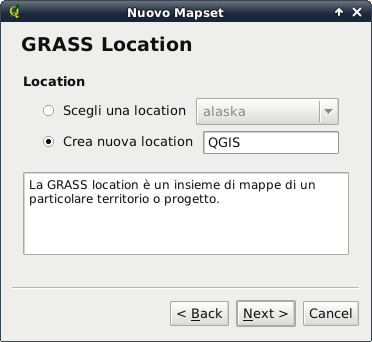
\includegraphics[clip=true, width=10cm]{create_grass_location}
\end{center}  
\end{figure}

\begin{enumerate}
  %\item Start QGIS and make sure the GRASS plugin is loaded
  \item Démarrez QGIS et assurez vous que l'extension GRASS est chargée.
  %\item Visualize the \filename{alaska.shp} Shapefile (see Section \ref{sec:load_shapefile}) from the QGIS alaska dataset~\ref{label_sampledata}.
  \item Affichez le shapefile \filename{alaska.shp} (voir Section \ref{sec:load_shapefile}) du jeu de données QGIS alaska ~\ref{label_sampledata}.
  %\item In the GRASS toolbar, click on the \toolbtntwo{grass_new_mapset}{Open mapset} icon to bring up the \filename{MAPSET} wizard.
  \item Dans la barre d'outils GRASS, cliquez sur \toolbtntwo{grass_new_mapset}{Nouveau jeu de données} pour ouvrir l'assistant \filename{Jeux de données}.
  %\item Select an existing GRASS database (GISDBASE) folder \filename{grassdata} or create one for the new \filename{LOCATION} using a file manager on your computer. Then click \button{Next}. 
  \item Sélectionnez un répertoire existant de base de données GRASS (Base de données) \filename {grassdata} ou créez en un pour le nouveau \filename{SECTEUR} avec le gestionnaire de fichiers de votre ordinateur. Cliquez le bouton \button{Suivant}.
  %\item We can use this wizard to create a new \filename{MAPSET} within an existing \filename{LOCATION} (see Section~\ref{sec:add_mapset}) or to create a new \filename{LOCATION} altogether. Click on the radio button \radiobuttonon{Create new location} (see Figure \ref{fig:create_grass_location}).
  \item Nous pouvons utiliser cet assistant à la fois pour créer un nouveau \filename{Jeu de données} dans un \filename{SECTEUR} existant (voir Section~\ref{sec:add_mapset}) et pour créer un nouveau \filename{SECTEUR}. Cliquez sur le bouton radio \radiobuttonon{Créez un nouveau secteur} (voir Figure \ref{fig:create_grass_location}).
  %\item Enter a name for the \filename{LOCATION} - we used alaska and click 
  \item Entrez un nom pour le \filename{SECTEUR} - nous utilisons alaska et cliquez sur le bouton \button{Suivant} 
  %\button{Next} 
  %\item Define the projection by clicking on the radio button \radiobuttonon{Projection} to enable the projection list 
  \item Définissez la projection en cliquant sur le bouton radio \radiobuttonon{Projection} pour activer la liste des projections
  %\item We are using Albers Equal Area Alaska (feet) projection. Since we happen to know that it is represented by the EPSG ID 2964, we enter it in
  %the search box. (Note: If you want to repeat this process for another  \filename{LOCATION} and projection and haven't memorized the EPSG ID, 
  %click on the \toolbtntwo{mIconProjectionEnabled}{projector} icon in the lower right-hand  corner of the status bar (see Section \ref{label_projstart})).
  \item Nous utilisons la projection Albers Equal Area Alaska (pieds).Étant donné que nous savons qu'elle correspond au code EPSG 2964, nous le saisissons dans le champ de recherche. (Note : Si vous souhaitez reproduire la manipulation pour un autre \filename{SECTEUR} et une autre projection et que vous ne connaissez pas le code EPSG, cliquez sur \toolbtntwo{mIconProjectionEnabled}{Statut de la projection} dans le coin inférieur droit de la barre d'état (voir Section \ref{label_projstart})).
  %\item Click \button{Find} to select the projection
  \item Cliquez sur \button{Trouver} pour sélectionner la projection
  %\item Click \button{Next} 
  \item Cliquer sur \button{Suivant} 
  %\item To define the default region, we have to enter the \filename{LOCATION} bounds in north, south, east, and west direction. Here we simply click on the button \button{Set current QGIS extent}, to apply the extend of the loaded layer \filename{alaska.shp} as the GRASS default region extend.
  \item Pour définir la région par défaut, nous devons saisir les limites Nord, Sud , Est et Ouest du \filename{SECTEUR}. Ici il suffit de cliquer sur le bouton \button{Fixer l'emprise courante de QGIS}, pour appliquer l'emprise du shapefile \filename{alaska.shp} déjà chargé comme emprise par défaut.
  %\item Click \button{Next} 
  \item Cliquer sur \button{Suivant} 
  %\item We also need to define a \filename{MAPSET} within our new \filename{LOCATION}. You can name it whatever you like - we used demo.\footnote{When creating a new \filename{LOCATION}, GRASS automatically creates a special \filename{MAPSET} called \filename{PERMANENT} designed to store the core data for the project, its default spatial extend and coordinate system definitions (Neteler \& Mitasova 2008  \cite{neteler_mitasova08}).}
  \item Nous avons aussi besoin de définir un \filename{Jeu de données} dans notre nouveau \filename{SECTEUR}. Vous pouvez l'appeler comme vous le souhaitez - nous utiliserons demo. \footnote{Quand nous créons un nouveau \filename{SECTEUR}, GRASS créé automatiquement un \filename{Jeu de données} spécial appelé \filename{PERMANENT} conçu pour stocker les données essentiels du projet, l'extension spatiale par défaut et la définition du système de coordonnées (Neteler \& Mitasova 2008  \cite{neteler_mitasova08}).}
  %\item Check out the summary to make sure it's correct and click \button{Finish} 
  \item Vérifiez le résumé pour vous assurez que tout est correct et cliquez sur \button{Terminer} 
  %\item The new \filename{LOCATION alaska} and two \filename{MAPSETs demo} and \filename{PERMANENT} are created. The currently opened working set is \filename{MAPSET demo}, as you defined.
  \item Le nouveau \filename{SECTEUR alaska} et les deux \filename{Jeux de données demo} et \filename{PERMANENT} sont créés. Actuellement, le jeu de données courant est le \filename{Jeux de données demo}, tel que vous l'avez défini.
  %\item Notice that some of the tools in the GRASS toolbar that were disabled are now enabled.
  \item Notez que certains outils qui n'étaient pas accessibles le sont maintenant.
\end{enumerate}

%If that seemed like a lot of steps, it's really not all that bad and a very quick way to create a \filename{LOCATION}. The \filename{LOCATION alaska} is 
%now ready for data import (see Section \ref{sec:import_loc_data}).You can also use the already existing vector and raster data in the sample 
%GRASS \filename{LOCATION alaska} included in the QGIS alaska dataset \ref{label_sampledata} and move on to Section \ref{label_vectmodel}.

Si cela semble faire beaucoup d'étapes, mais c'est en fait un moyen simple et rapide de créer un \filename{SECTEUR}. Le \filename{SECTEUR alaska} est maintenant prêt pour l'importation de données (voir Section \ref{sec:import_loc_data}). Vous pouvez également utiliser des données raster ou vecteur existantes dans le \filename{SECTEUR alaska} inclues dans le jeu de données QGIS alaska \ref{label_sampledata} et continuez dans la section \ref{label_vectmodel}.

%\subsubsection{Adding a new MAPSET}\label{sec:add_mapset}
\subsubsection{Ajouter un nouveau Jeu de données}\label{sec:add_mapset}

%A user has only write access to a GRASS \filename{MAPSET} he created. This means, besides access to his own \filename{MAPSET}, each user can also read 
%maps in other user's \filename{MAPSETs}, but he can modify or remove only the maps in his own \filename{MAPSET}. All \filename{MAPSETs} include a 
%\filename{WIND} file that stores the current boundary coordinate values and the currently selected raster resolution (Neteler \& Mitasova 2008 \cite{neteler_mitasova08}, see Section \ref{sec:grass_region}). 

Un utilisateur a seulement des droits d'écriture sur le \filename{Jeu de données} GRASS qu'il a créé. Cela veut dire qu'au delà de l'accès à son propre \filename{Jeu de données} GRASS, chaque utilisateur peut aussi lire les données dans les autres \filename{Jeux de données}, mais il ne peut modifier et supprimer que les données que dans son propre \filename{Jeu de données}. Tous les \filename{Jeux de données} incluent un fichier \filename{WIND} qui stocke l'extension et la résolution raster courante (Neteler \& Mitasova 2008 \cite{neteler_mitasova08}, voir Section \ref{sec:grass_region}). 


\begin{enumerate}
  %\item Start QGIS and make sure the GRASS plugin is loaded
  \item Démarrer QGIS et assurez vous que l'extension GRASS est chargée
  %\item In the GRASS toolbar, click on the \toolbtntwo{grass_new_mapset}{New mapset} icon to bring up the \filename{MAPSET} wizard.
  \item Dans la barre d'outils GRASS, cliquez sur \toolbtntwo{grass_new_mapset}{Nouveau jeu de données} pour ouvrir l'assistant \filename{Jeux de données}.
  %\item Select the GRASS database (GISDBASE) folder \filename{grassdata}  with the \filename{LOCATION alaska}, where we want to add a further \filename{MAPSET}, called test.
  \item Sélectionnez le répertoire \filename{grassdata} de la base de données GRASS (Base de données) qui contient déjà le \filename{SECTEUR alaska} et où nous voulons ajouter un autre \filename{SECTEUR} appelé test.
  %\item Click \button{Next}. 
  \item Cliquez sur \button{Suivant}. 
  %\item We can use this wizard to create a new \filename{MAPSET} within an existing \filename{LOCATION} or to create a new \filename{LOCATION} altogether. Click on the radio button \radiobuttonon{Select location} (see Figure \ref{fig:create_grass_location}) and click \button{Next}.
  \item Nous pouvons utiliser cet assistant à la fois pour créer un nouveau \filename{Jeu de données} dans le \filename{SECTEUR} existant et pour créer un nouveau \filename{SECTEUR}. Cliquez sur le bouton radio \radiobuttonon{Sélectionnez le Secteur} (voir Figure \ref{fig:create_grass_location}) et cliquez sur \button{Suivant}.
  %\item Enter the name \filename{text} for the new \filename{MAPSET}. Below in the wizard you see a list of existing \filename{MAPSETs} and its owners.
  \item Entrez le \filename{text} du nom pour le nouveau \filename{Jeu de données}. En dessous, dans l'assistant, vous pouvez voir une liste des \filename{Jeux de données} et de leurs propriétaires.
  %\item Click \button{Next}, check out the summary to make sure it's all correct and click \button{Finish}
  \item Cliquez sur \button{Suivant}, vérifiez le résumé pour vous assurer qu'il est correct et cliquez sur \button{Terminer} 
\end{enumerate}

%\subsection{Importing data into a GRASS LOCATION}\label{sec:import_loc_data}
\subsection{Importer des données dans un SECTEUR GRASS}\label{sec:import_loc_data}
%This Section gives an example how to import raster and vector data into the \filename{alaska} GRASS \filename{LOCATION} provided by the QGIS alaska dataset.
%Therefore we use a landcover raster map \filename{landcover.img} and a vector GML File \filename{lakes.gml} from the QGIS alaska dataset \ref{label_sampledata}.
Cette section donne un exemple d'importation de données raster et vecteur dans le \filename{SECTEUR} GRASS \filename{alaska} fournit dans le jeu de données QGIS alaska. Nous utiliserons une couche raster d'occupation du sol \filename{landcover.img} et une couche vecteur au format GML \filename{lakes.gml}, toutes deux présentes dans le jeu de données alaska.
\begin{enumerate}
  %\item Start QGIS and make sure the GRASS plugin is loaded.
  \item Démarrer QGIS et assurez vous que l'extension GRASS est chargée.
  %\item In the GRASS toolbar, click the \toolbtntwo{grass_open_mapset}{Open MAPSET} icon to bring up the \filename{MAPSET} wizard.
  \item Dans la barre d'outil GRASS, cliquez sur \toolbtntwo{grass_open_mapset}{Ouvrir un jeu de données} pour ouvrir l'assistant \filename{Jeu de données}.
  %\item Select as GRASS database the folder \filename{grassdata} in the QGIS alaska dataset, as \filename{LOCATION alaska}, as \filename{MAPSET} 
  %\filename{demo} and click \button{OK}.
  \item Sélectionnez comme base de données GRASS le répertoire \filename{grassdata} dans le jeu de données QGIS alaska, comme \filename{SECTEUR alaska}, comme as \filename{Jeu de donnée} \filename{demo} et cliquez sur \button{OK}.
  %\item Now click the \toolbtntwo{grass_tools}{Open GRASS tools} icon. The GRASS Toolbox (see Section \ref{subsec:grass_toolbox}) dialog appears.
  \item Maintenant cliquez sur \toolbtntwo{grass_tools}{Ouvrir les outils GRASS}. La boîte à outils GRASS (voir Section \ref{subsec:grass_toolbox}) s'ouvre.
  %\item To import the raster map \filename{landcover.img}, click the module \filename{r.in.gdal} in the \tab{Modules Tree} tab. This GRASS module allows to import GDAL supported raster files into a GRASS \filename{LOCATION}. The module dialog for \filename{r.in.gdal} appears.
  \item  Pour importer la couche raster \filename{landcover.img}, cliquez sur le module \filename{r.in.gdal} dans l'onglet \tab{Arborescence des modules}. Ce module GRASS vous permet d'importer les fichiers raster supportés par la librairie GDAL dans un \filename{SECTEUR} GRASS. La boîte de dialogue  \filename{r.in.gdal} apparaît.
  %\item Browse to the folder \filename{raster} in the QGIS alaska dataset and select the file \filename{landcover.img}.
  \item Naviguer jusqu'au répertoire \filename{raster} dans le jeu de données QGIS alaska et sélectionnez le fichier \filename{landcover.img}.
  %\item As raster output name define \filename{landcover\_grass} and click \button{Run}. In the \tab{Output} tab you see the currently running GRASS command \filename{r.in.gdal -o input=/path/to/landcover.img output=landcover\_grass}.
  \item Définissez \filename{landcover\_grass} comme nom de sortie et cliquez sur \button{Lancer}. Dans l'onglet \tab{Rendu}, vous voyez la commande GRASS en cours \filename{r.in.gdal -o input=/path/to/landcover.img output=landcover\_grass}.
  %\item When it says \textbf{Succesfully finished} click \button{View output}. 
  \item Lorsque \textbf{Terminé avec succès} s'affiche cliquez sur \button{Vue}. 
  %The \filename{landcover\_grass} raster layer is now imported into GRASS and will be visualized in the QGIS canvas.
  La couche raster \filename{landcover\_grass} est maintenant importée dans GRASS et pourra être affichée dans QGIS.
  
  %\item To import the vector GML file \filename{lakes.gml}, click the module \filename{v.in.ogr} in the \tab{Modules Tree} tab. This GRASS module allows to import OGR supported vector files into a GRASS \filename{LOCATION}. The module dialog for \filename{v.in.ogr} appears.
  \item Pour importer le fichier GML \filename{lakes.gml}, cliquez sur le module \filename{v.in.ogr} dans l'onglet \tab{Arborescence des modules}.La boîte de dialogue  \filename{v.in.ogr} apparaît.
  %\item Browse to the folder \filename{gml} in the QGIS alaska dataset and select the file \filename{lakes.gml} as OGR file.
  \item Naviguer jusqu'au répertoire \filename{gml} dans le jeu de données QGIS alaska et sélectionnez le fichier \filename{lakes.gml}.
  %\item As vector output name define \filename{lakes\_grass} and click \button{Run}. You don't have to care about the other options in this   example. In the \tab{Output} tab you see the currently running GRASS command \filename{v.in.ogr -o dsn=/path/to/lakes.gml output=lakes\_grass}.
  \item Définissez \filename{lakes\_grass} comme nom de sortie et cliquez sur \button{Lancer}. Vous n'avez pas besoin des autres options dans cet exemple.
  %\item When it says \textbf{Succesfully finished} click \button{View output}. 
  \item Lorsque \textbf{Terminé avec succès} s'affiche cliquez sur \button{Vue}. 
  %The \filename{lakes\_grass} vector layer is now imported into GRASS and will be visualized in the QGIS canvas. 
  Le fichier \filename{lakes\_grass} est maintenant importé dans GRASS et pourra être affiché dans QGIS.
\end{enumerate}


%\subsection{The GRASS vector data model}\label{label_vectmodel}\index{GRASS!vector datamodel}
\subsection{Le modèle vecteur de GRASS}\label{label_vectmodel}\index{GRASS!modèle vecteur}
%It is important to understand the GRASS vector data model prior to digitizing.\index{GRASS!digitizing} In general, GRASS uses a topological vector model.\index{GRASS!topology} This means that areas are not represented as closed polygons, but by one or more boundaries. A boundary between two adjacent areas is digitized only once, and it is shared by both areas. Boundaries must be connected without gaps. An area is identified (labeled) by the centroid of the area.
Il est important de comprendre le modèle vecteur de GRASS avant de faire de la numérisation.\index{GRASS!numérisation} En général, GRASS utilise un modèle vecteur topologique.\index{GRASS!topologie} Cela veut dire que les surfaces ne sont pas représentées par des polygones fermés mais par une ou plusieurs limites. Une limite entre des polygones adjacents n'est numérisée qu'une seule fois et est partagée par les deux surfaces. Les limites doivent être connectées sans trous. Une surface est identifiée (libellée) via le centroide de la surface.

%Besides boundaries and centroids, a vector map can also contain points and lines. All these geometry elements can be mixed in one vector and will be represented in different so called 'layers' inside one GRASS vector map. So in GRASS a layer is not a vector or raster map but a level inside a vector layer. This is important to distinguish carefully.
	
Outre les limites et centro"ides, une couche vecteur peut également contenir des points et des lignes. Tous ces éléments de géométrie peuvent être mélangés dans une couche vecteur et seront représentés dans différentes «sous-couches» dans une carte vectorielle GRASS. Ainsi, une couche GRASS n'est pas un vecteur ou un raster, mais un niveau à l'intérieur d'une couche vecteur. Il est important de bien distinguer ceci.

%\footnote{Although it is possible to mix geometry elements, it is unusual and even in GRASS only used in special cases such as vector network analysis. Normally you should
%prefere to store different geometry elements in different layers.}
\footnote{Même s'il est possible de mélanger des éléments de géométries différentes, c'est inhabituel et même dans GRASS, on l'utilise dans des cas particuliers tel que l'analyse de réseau. Normalement, vous devriez stocker des éléments de géométries différentes dans des couches différentes}

%It is possible to store more 'layers' in one vector dataset. For example, fields, forests and lakes can be stored in one vector. Adjacent forest and lake can share the same boundary, but they have separate attribute tables. It is also possible to attach attributes to boundaries. For example, the boundary between lake and forest is a road, so it can have a different attribute table.
Il est possible de stocker plusieurs sous-couches dans une couche vecteur. Par exemple, des champs, de la forêt et des lacs peuvent être stockés dans une couche vecteur. Les forêts et les lacs adjacents partagent les mêmes limites, mais ils auront des tables attributaires différentes. Il est aussi possible de faire correspondre une table attributaires aux limites. Par exemple, la limite entre un lac et une forêt peut être une route qui peut avoir une table attributaire différente.

%The 'layer' of the feature is defined by 'layer' inside GRASS. 'Layer' is the number which defines if there are more than one layer inside the dataset, e.g. if the geometry is forest or lake. For now, it can be only a number, in the future GRASS will also support names as fields in the user interface.
La 'sous-couche' est définie dans GRASS par un chiffre. Ce chiffre définit s'il y a plusieurs sous-couches à l'intérieur d'une couche vecteur. Par exemple, il définit s'il s'agit de lac ou de forêt. Pour l'instant, il s'agit d'un nombre mais dans des versions futures GRASS pourra utiliser des noms pour les sous-couches dans l'interface utilisateur.

%Attributes can be stored inside the GRASS \filename{LOCATION} as DBase or SQLITE3 or in external database tables, for example PostgreSQL, MySQL, Oracle, etc.\index{GRASS!attribute storage}
Les données attributaires peuvent être stockées dans le \filename{SECTEUR} au format DBase ou SQLIte3 ou dans des tables de bases de données externes comme par exemple : PostgreSQL, MySQL, Oracle, etc.\index{GRASS!stockage des attributs}

%Attributes in database tables are linked to geometry elements using a 'category' value.\index{GRASS!attribute linkage} 'Category' (key, ID) is an
%integer attached to geometry primitives, and it is used as the link to one key column in the database table.
Les données attributaires sont liées à la géométrie par le biais d'un champ 'category'.\index{GRASS!liens des attributs} 'Category' (clé, ID) est un entier attaché à la géométrie, et il est utilisé comme lien vers une colonne de clé dans la table de base de données.


%\begin{Tip}\caption{\textsc{Learning the GRASS Vector Model}}
\begin{Astuce}\caption{\textsc{Apprendre le modèle vecteur de GRASS}}
\qgistip{
%The best way to learn the GRASS vector model and its capabilities is to download one of the many GRASS tutorials where the vector model is described
%more deeply. See \url{http://grass.osgeo.org/gdp/manuals.php} for more information, books and tutorials in several languages.
Le meilleur moyen d'apprendre le modèle vecteur de GRASS et ses possibilités est de télécharger un des nombreux tutoriels GRASS où le modèle vecteur est décrit plus précisément. Voir \url{http://grass.osgeo.org/gdp/manuals.php} pour des informations complémentaires, des livres et des tutoriels dans différentes langues.
}
\end{Astuce} 

%\subsection{Creating a new GRASS vector layer}\label{sec:creating_new_grass_vectors}\index{GRASS!Creating new vectors|see{editing!creating a new layer}}
\subsection{Création d'une nouvelle couche vecteur GRASS}\label{sec:creating_new_grass_vectors}\index{GRASS!Créer de nouvelles couches vecteur|voir{éditer!créer une nouvelle couche}}

%To create a new GRASS vector layer with the GRASS plugin click the \toolbtntwo{grass_new_vector_layer}{Create new GRASS vector} toolbar icon. 
%Enter a name in the text box and you can start digitizing point, line or polygone geometries, following the procedure described in Section \ref{grass_digitising}. 
Pour créer une nouvelle couche vecteur GRASS à l'aide de l'extension GRASS, cliquez sur \toolbtntwo{grass_new_vector_layer}{Créez une nouvelle couche vectorielle GRASS} dans la barre d'outils. Entrez le nom dans la boîte de dialogue et vous pouvez commencer à digitaliser un point une ligne ou un polygone en suivant les instructions de la section \ref{grass_digitising}.
%In GRASS it is possible to organize all sort of geometry types (point, line and area) in one layer, because GRASS uses a topological vector model, so you don't need to select the geometry type when creating a new GRASS vector. This is different from Shapefile creation with QGIS, because Shapefiles use the Simple Feature vector model (see Section \ref{sec:create shape}).
Dans GRASS, il est possible de gérer plusieurs types de géométrie (point, ligne et surface) dans une seule couche d'information, car GRASS utilise un modèle vecteur topologique. Vous n'avez donc pas besoin de sélectionner un type de géométrie quand vous créez une couche vecteur GRASS. C'est différent de la création de shapefile avec QGIS, car les shapefiles utilisent un modèle vecteur d'entité simple (Simple Feature vector model) (voir Section \ref{sec:create shape}).

%\begin{Tip}\caption{\textsc{Creating an attribute table for a new GRASS vector layer}}
\begin{Astuce}\caption{\textsc{Création d'une table attributaire pour une nouvelle couche vecteur GRASS}}
\qgistip{
%If you want to assign attributes to your digitized geometry features, make sure to create an attribute table with columns before you start digitizing (see Figure \ref{fig:grass_digitizing_table}).
Si vous souhaitez renseigner les données attributaires de vos entités numérisées, assurez-vous d'avoir créé une table attributaire avec des champs avant ce commencer votre numérisation (voir Figure \ref{fig:grass_digitizing_table}).
}
\end{Astuce} 

%\subsection{Digitizing and editing a GRASS vector layer}\index{GRASS!digitizing tools}\label{grass_digitising}
\subsection{Numérisation et édition de couche vecteur GRASS}\index{GRASS!outils de numérisation}\label{grass_digitising}

%The digitizing tools for GRASS vector layers are accessed using the \toolbtntwo{grass_edit}{Edit GRASS vector layer} icon on the toolbar. Make 
%sure you have loaded a GRASS vector and it is the selected layer in the legend before clicking on the edit tool. Figure \ref{fig:grass_digitizing_category} shows the GRASS edit dialog that is displayed when you click on the edit tool. The tools and settings are discussed in the following sections.
Les outils de numérisation pour les couches vecteurs de GRASS sont accessibles via \toolbtntwo{grass_edit}{Éditer une couche vectorielle GRASS} dans la barre d'outils. Assurez-vous d'avoir ouvert une couche vectorielle GRASS ainsi que d'avoir sélectionné la sous-couche dans la légende avant d'utiliser l'outil d'édition. La figure \ref{fig:grass_digitizing_category} montre la boîte de dialogue GRASS qui s'affiche quand vous cliquez sur l'outil d'édition. Les outils et les paramètres d'édition sont détaillés dans les sections suivantes.

%\begin{Tip}\caption{\textsc{Digitizing polygones in GRASS}}
\begin{Astuce}\caption{\textsc{Numérisation de polygones dans GRASS}}
\qgistip{
%If you want to create a polygone in GRASS, you first digitize the boundary of the polygone, setting the mode to \usertext{No category}. Then you add a centroid (label point) into the closed boundary, setting the mode to \usertext{Next not used}. The reason is, that a topological vector model links attribute information of a polygon always to the centroid and not to the boundary.
Si vous voulez créer un polygone dans GRASS, vous devez numériser premièrement les limites du polygone, en définissant mode sur \usertext{Pas de catégorie}.Ensuite, vous ajoutez un centro"ide (emplacement de l'étiquette) dans le polygone fermé, fixant le mode sur \usertext{Prochain non utilisé}. La raison en est, que le modèle vectoriel topologique assure toujours le lien entre les informations d'attributs des polygones via le centro"ide et non via la limite.}
\end{Astuce} 

\minisec{Barre d'outils}\label{label_grasstoolbar}

%In Figure \ref{fig:grass_digitizing_toolbar} you see the GRASS digitizing toolbar icons provided by the GRASS plugin. Table \ref{tab:grass_tools}
%explains the available functionalities.
Sur la figure \ref{fig:grass_digitizing_toolbar} vous pouvez voir la barre d'outils d'édition GRASS de l'extension GRASS. Le tableau \ref{tab:grass_tools} récapitule les fonctions disponibles.

\begin{figure}[h]
   \begin{center}
%   \caption{GRASS Digitizing Toolbar \nixcaption}\label{fig:grass_digitizing_toolbar} 
   \caption{Barre d'outils d'édition GRASS \nixcaption}\label{fig:grass_digitizing_toolbar} 
   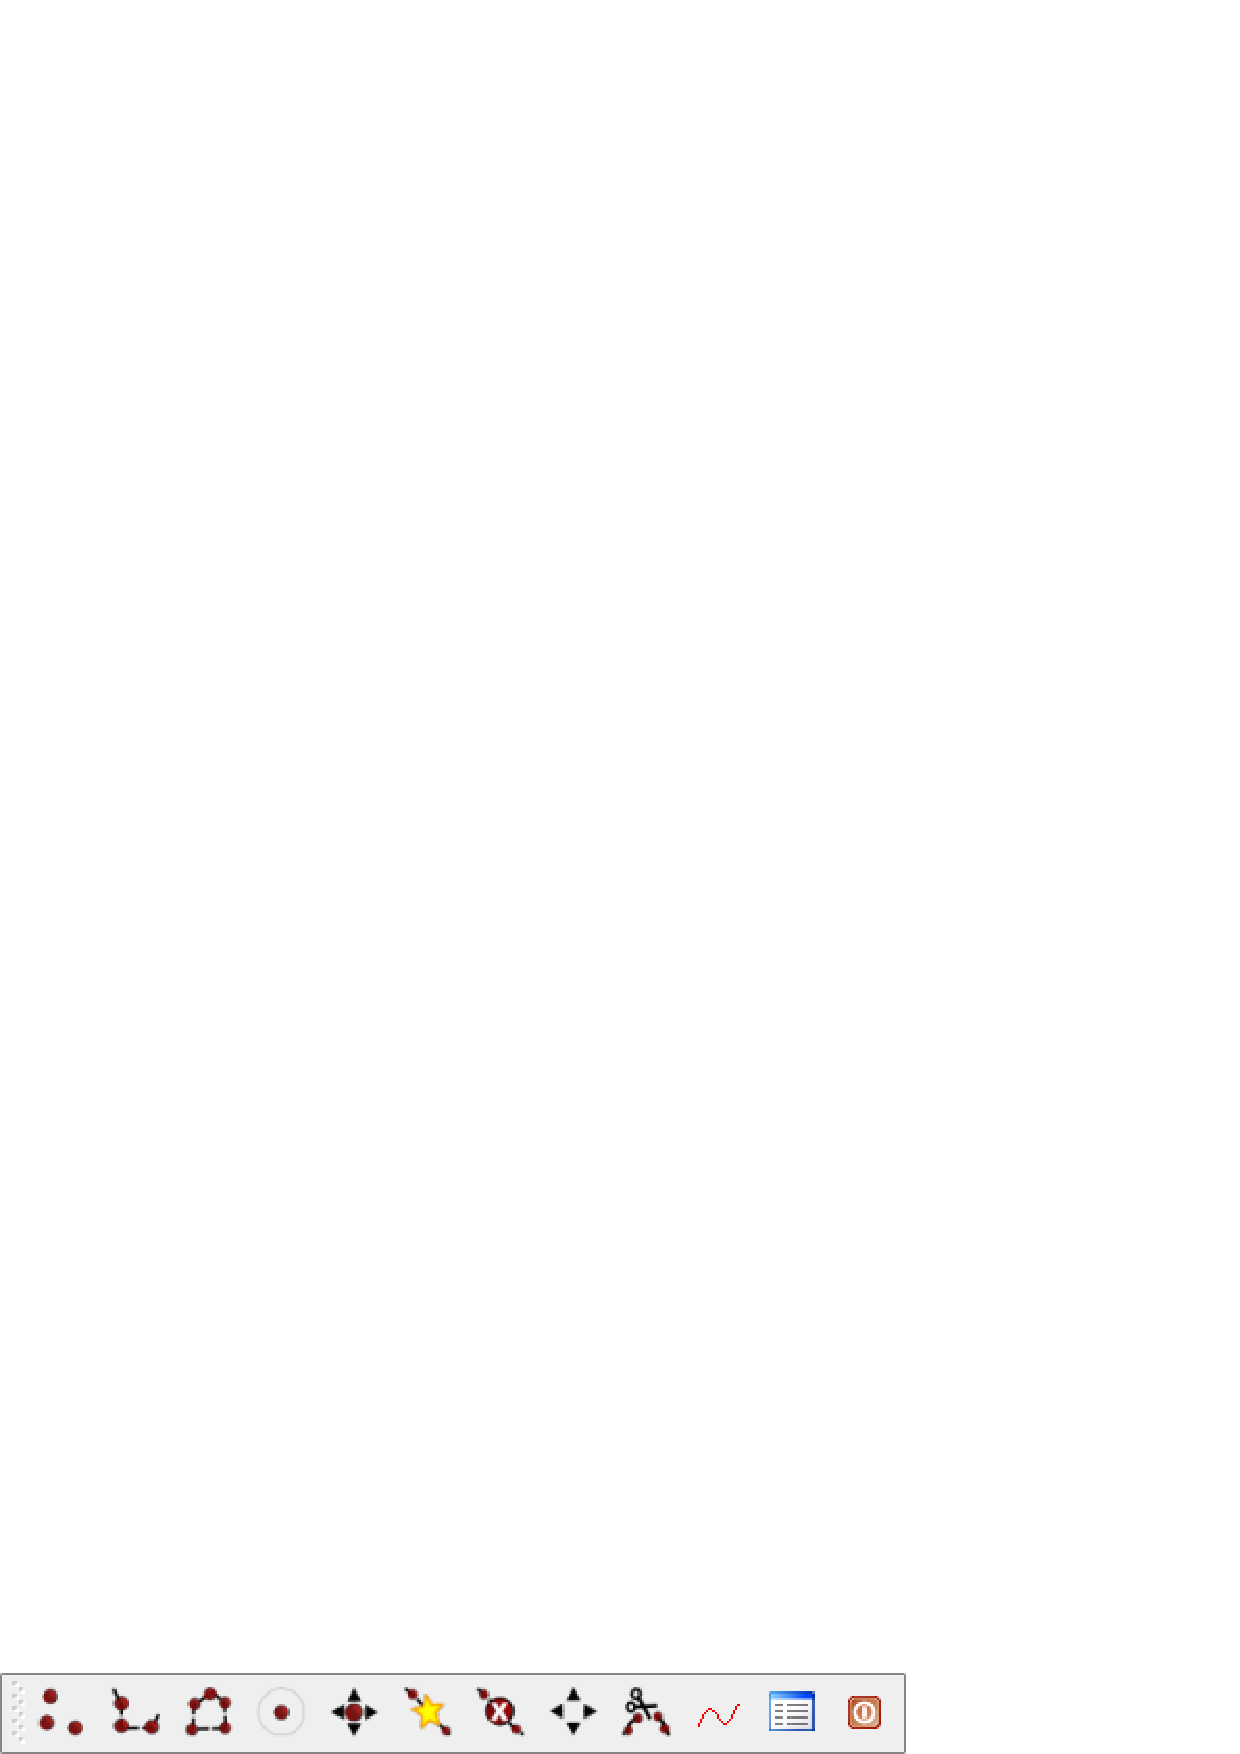
\includegraphics[clip=true,width=12cm]{grass_digitizing_toolbar}
\end{center}  
\end{figure}

%\begin{table}[h]\index{GRASS!digitizing tools}
\begin{table}[h]\index{GRASS!outils de numérisation}
\centering
%\caption{GRASS Digitizing Tools}\label{tab:grass_tools}\medskip
\caption{Outils de numérisation GRASS}\label{tab:grass_tools}\medskip
 \begin{tabular}{|l|l|p{5in}|}
%\hline \textbf{Icon} & \textbf{Tool} & \textbf{Purpose} \\
%\hline 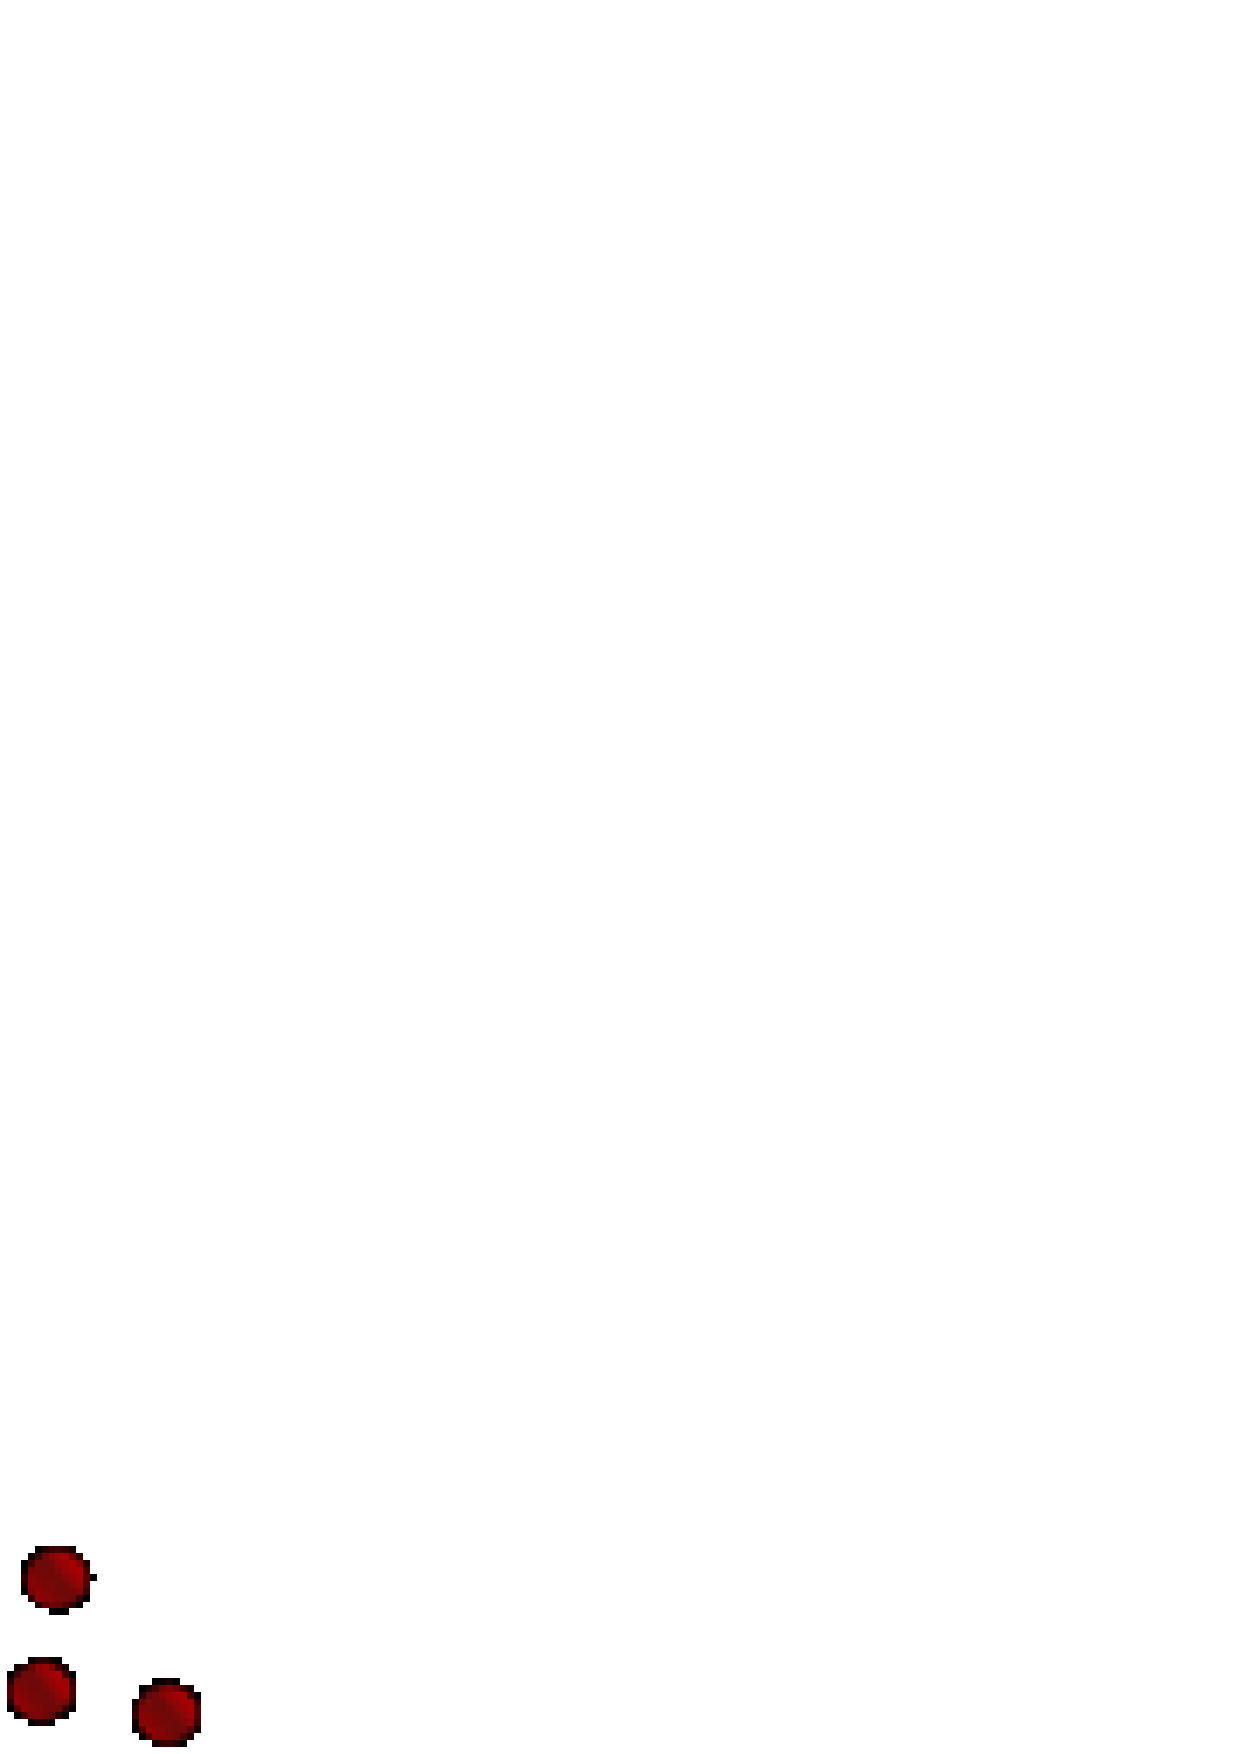
\includegraphics[width=0.7cm]{grass_new_point} & New Point & Digitize new point \\
%\hline 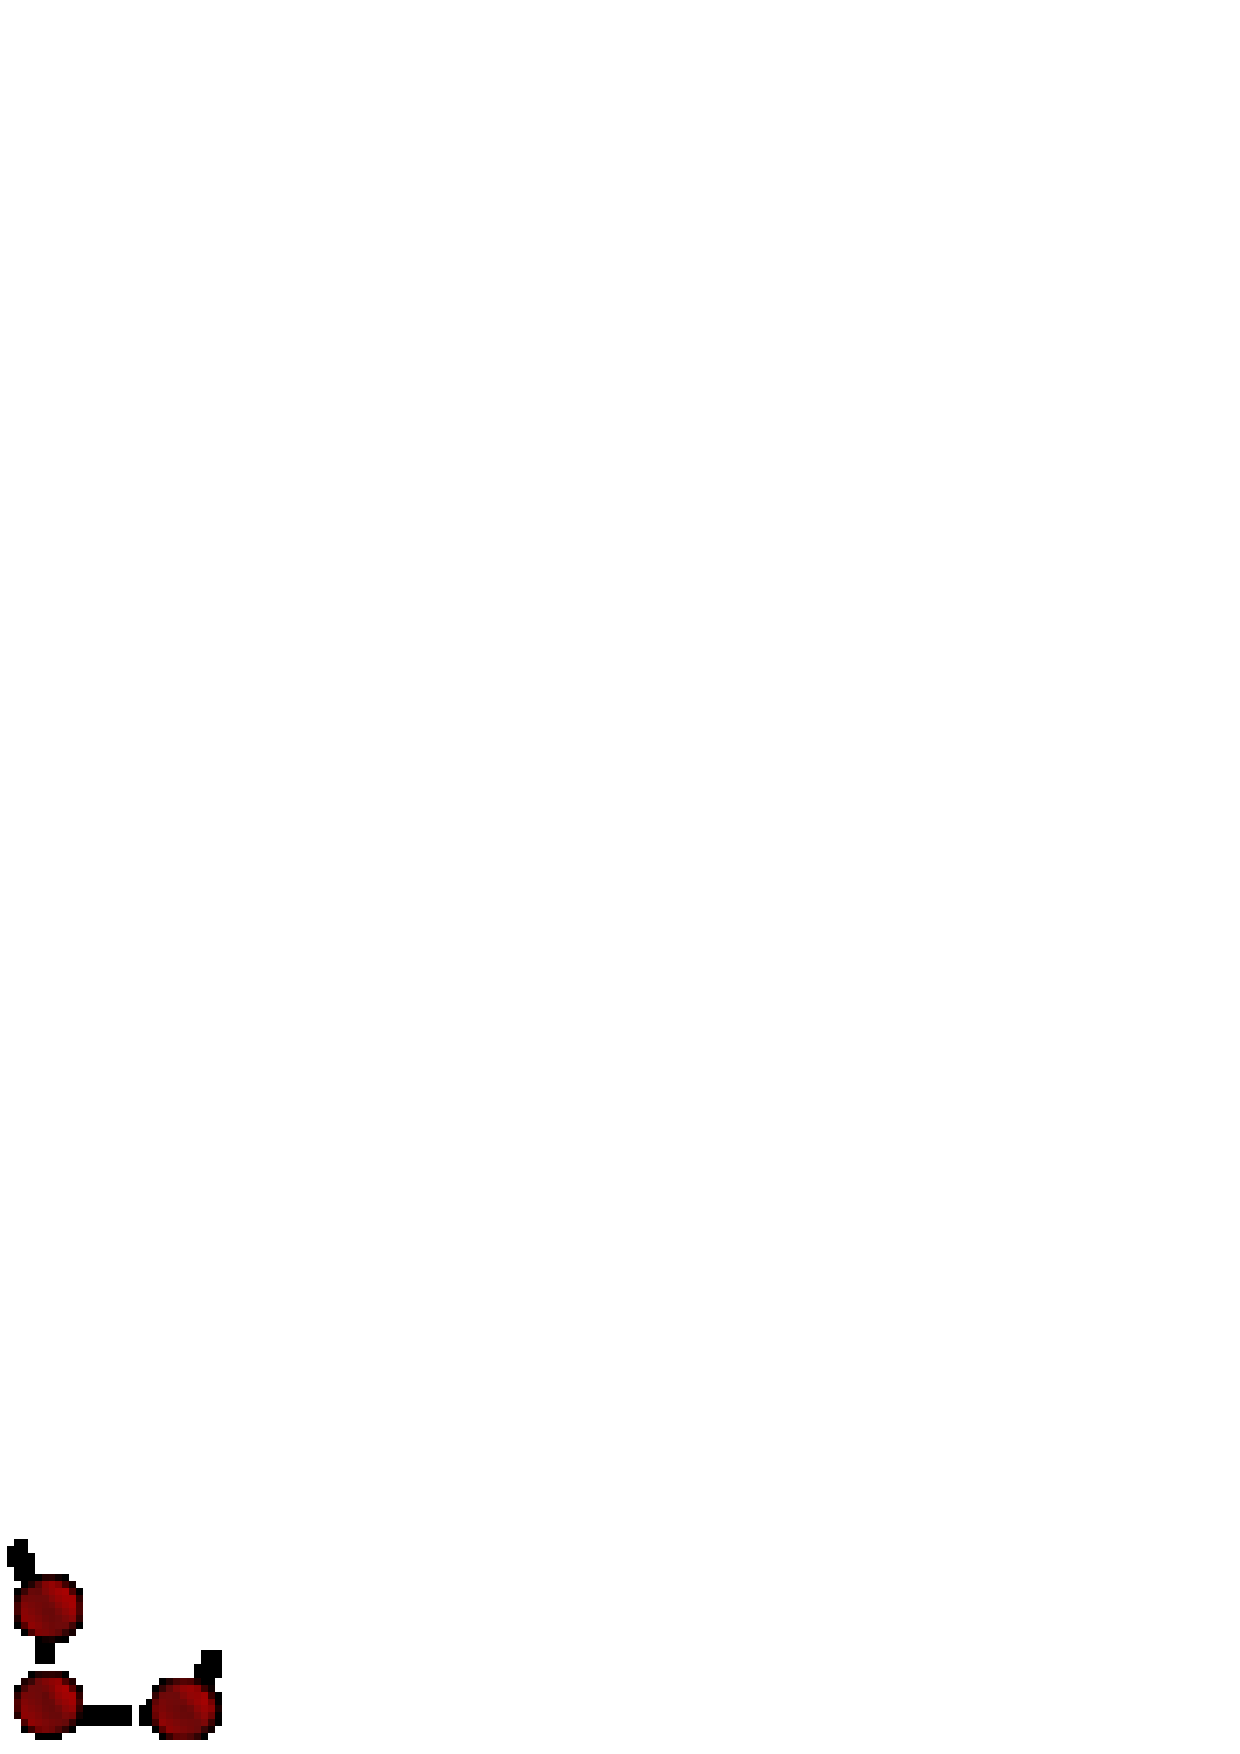
\includegraphics[width=0.7cm]{grass_new_line} & New Line & Digitize new line (finish by selecting new tool) \\
%\hline 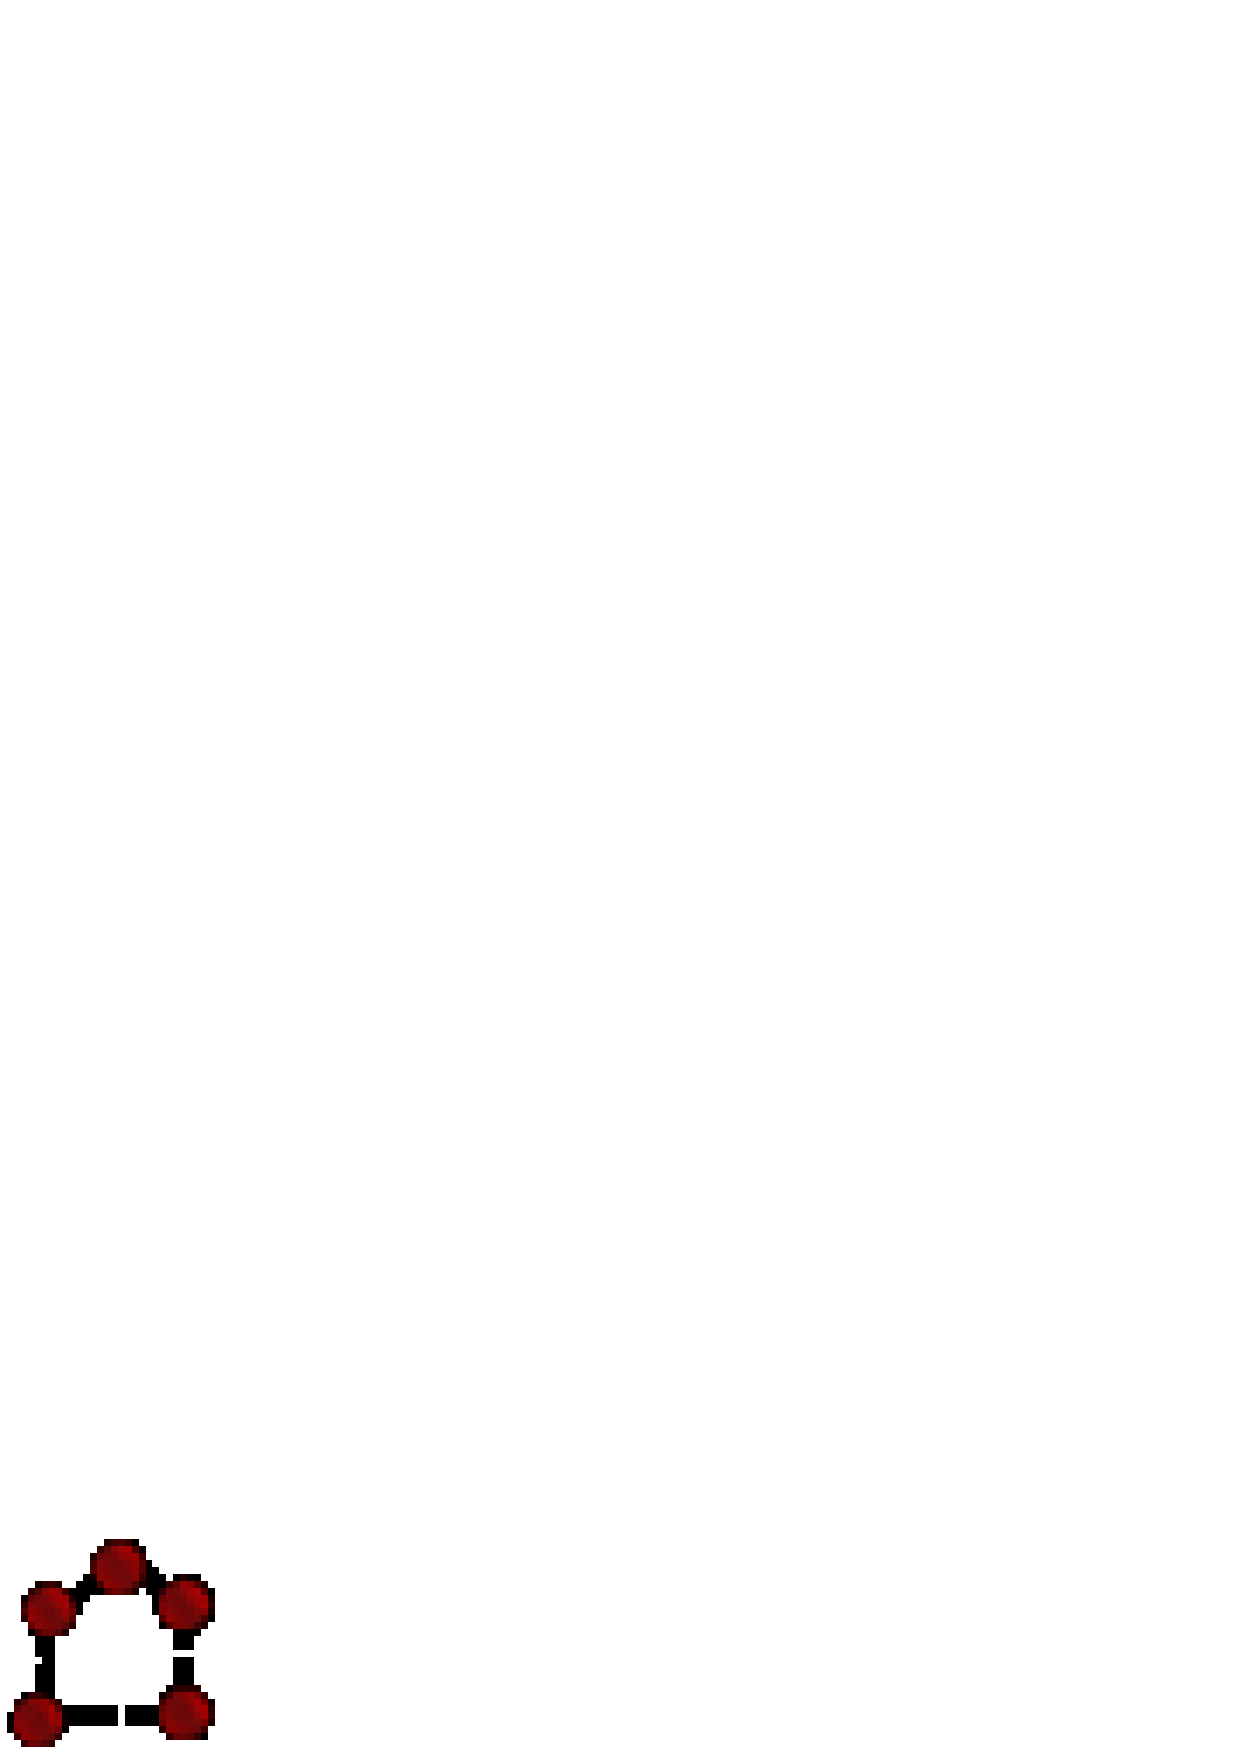
\includegraphics[width=0.7cm]{grass_new_boundary} & New Boundary & Digitize new boundary (finish by selecting new tool)\\
%\hline 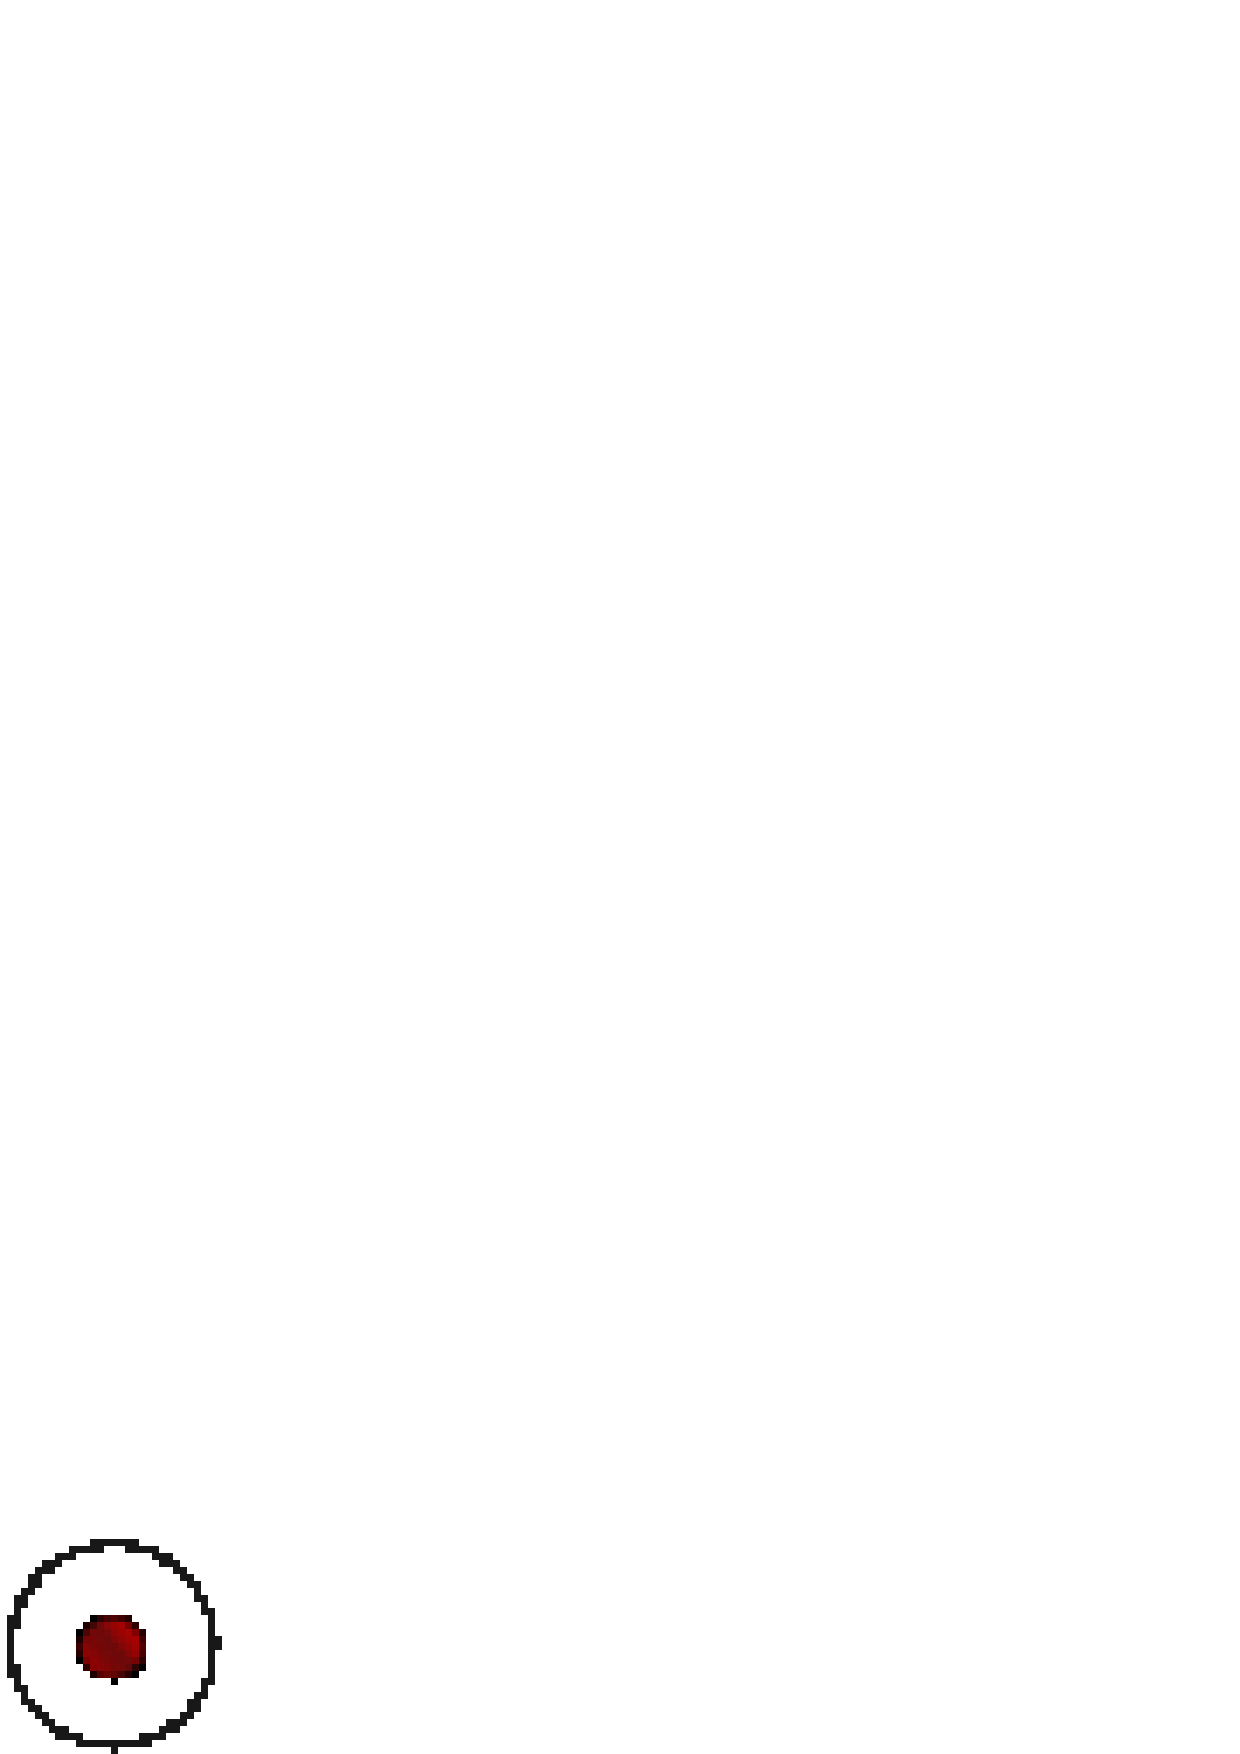
\includegraphics[width=0.7cm]{grass_new_centroid} & New Centroid & Digitize new centroid (label existing area)\\
%\hline 
\includegraphics[width=0.7cm]{grass_move_vertex} & Move vertex & Move one vertex of existing line or boundary and identify new position\\
%\hline 
\includegraphics[width=0.7cm]{grass_add_vertex} & Add vertex & Add a new vertex to existing line\\
%\hline 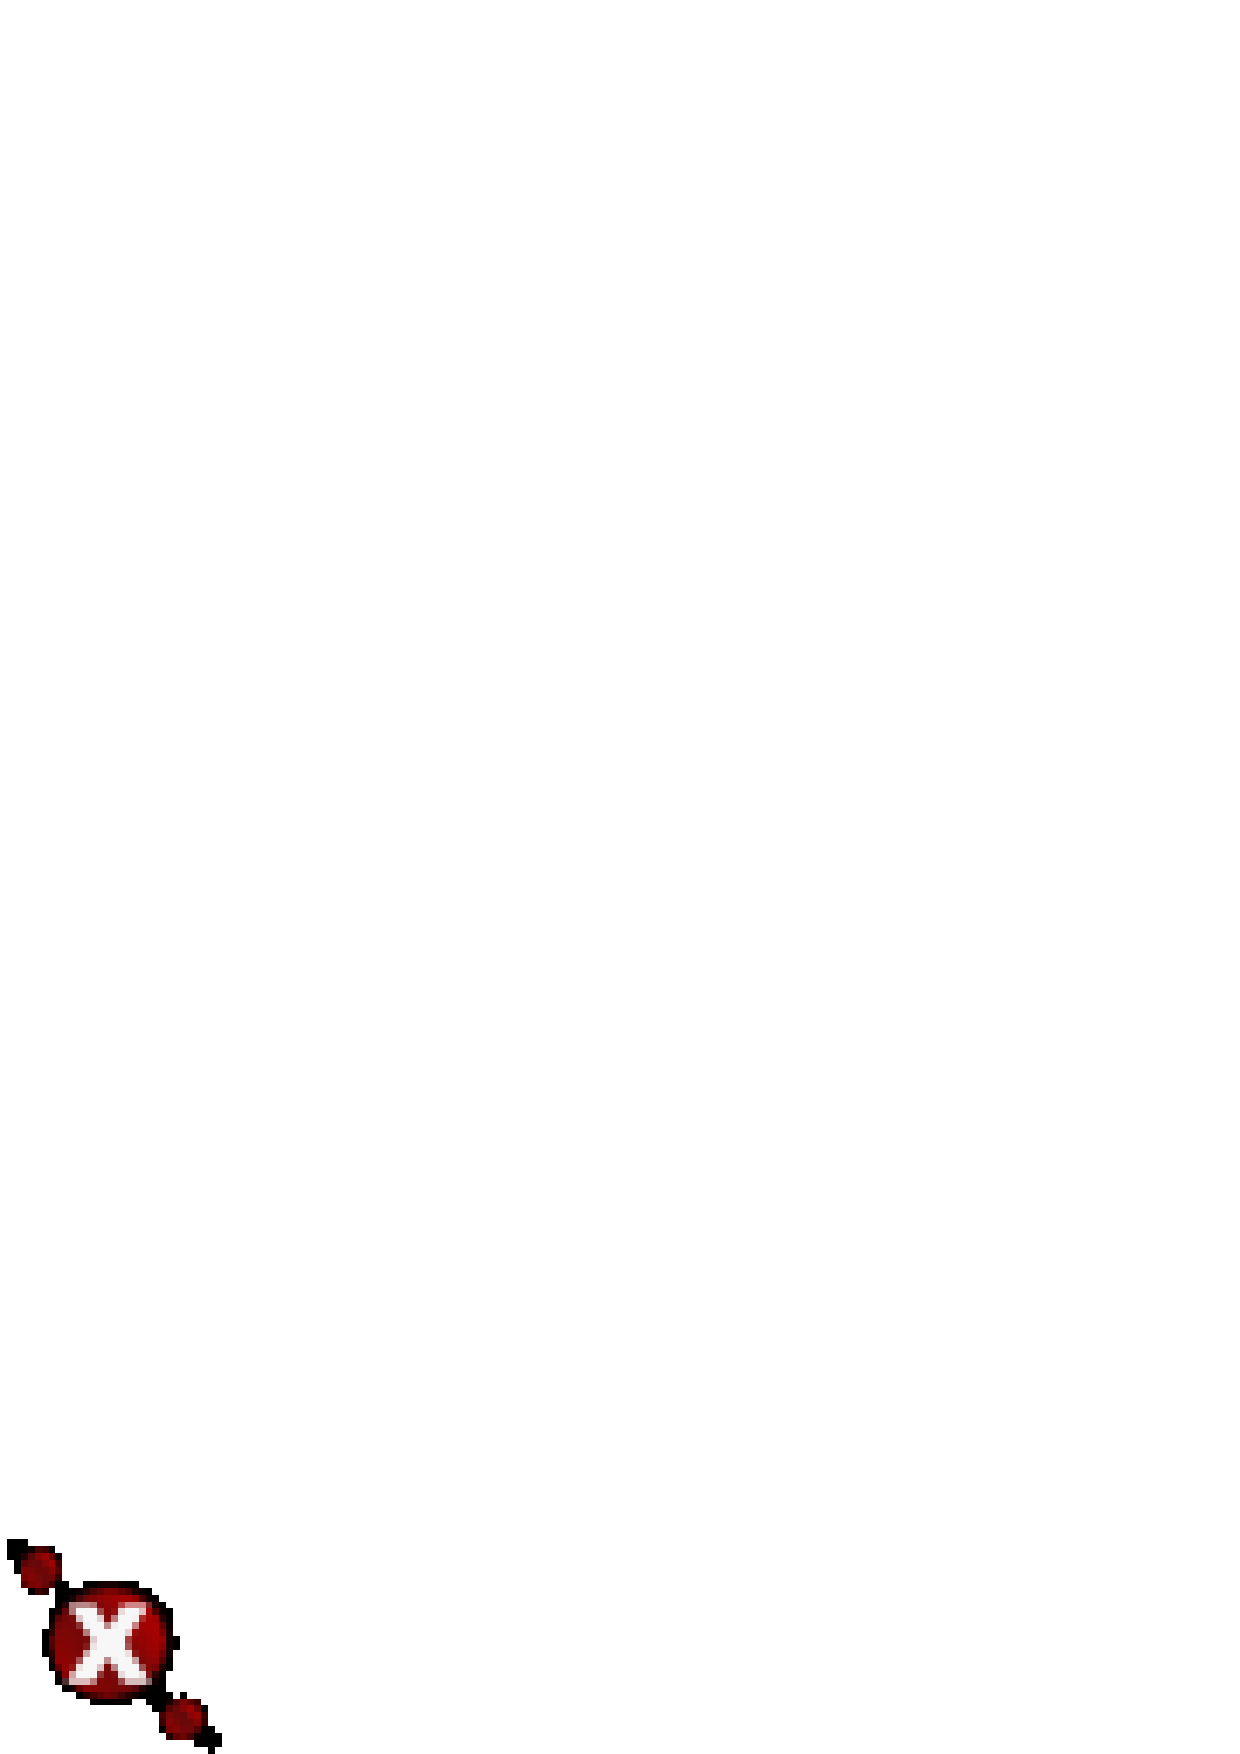
\includegraphics[width=0.7cm]{grass_delete_vertex} & Delete vertex & Delete vertex from existing line (confirm selected vertex by another click)\\
%\hline 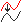
\includegraphics[width=0.7cm]{grass_move_line} & Move element & Move selected boundary, line, point or centroid and click on new position\\
%\hline 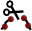
\includegraphics[width=0.7cm]{grass_split_line} & Split line & Split an existing line to 2 parts\\
%\hline 
\includegraphics[width=0.7cm]{grass_delete_line} & Delete element & Delete existing boundary, line, point or centroid (confirm selected element by another click)\\
%\hline 
\includegraphics[width=0.7cm]{grass_edit_attributes} & Edit attributes & Edit attributes of selected element (note that one element can represent more features, see above)\\
%\hline 
\includegraphics[width=0.7cm]{grass_close_edit} & Close & Close session and save current status (rebuilds topology afterwards)\\
\hline \textbf{Icône} & \textbf{Outil} & \textbf{Fonction} \\
\hline 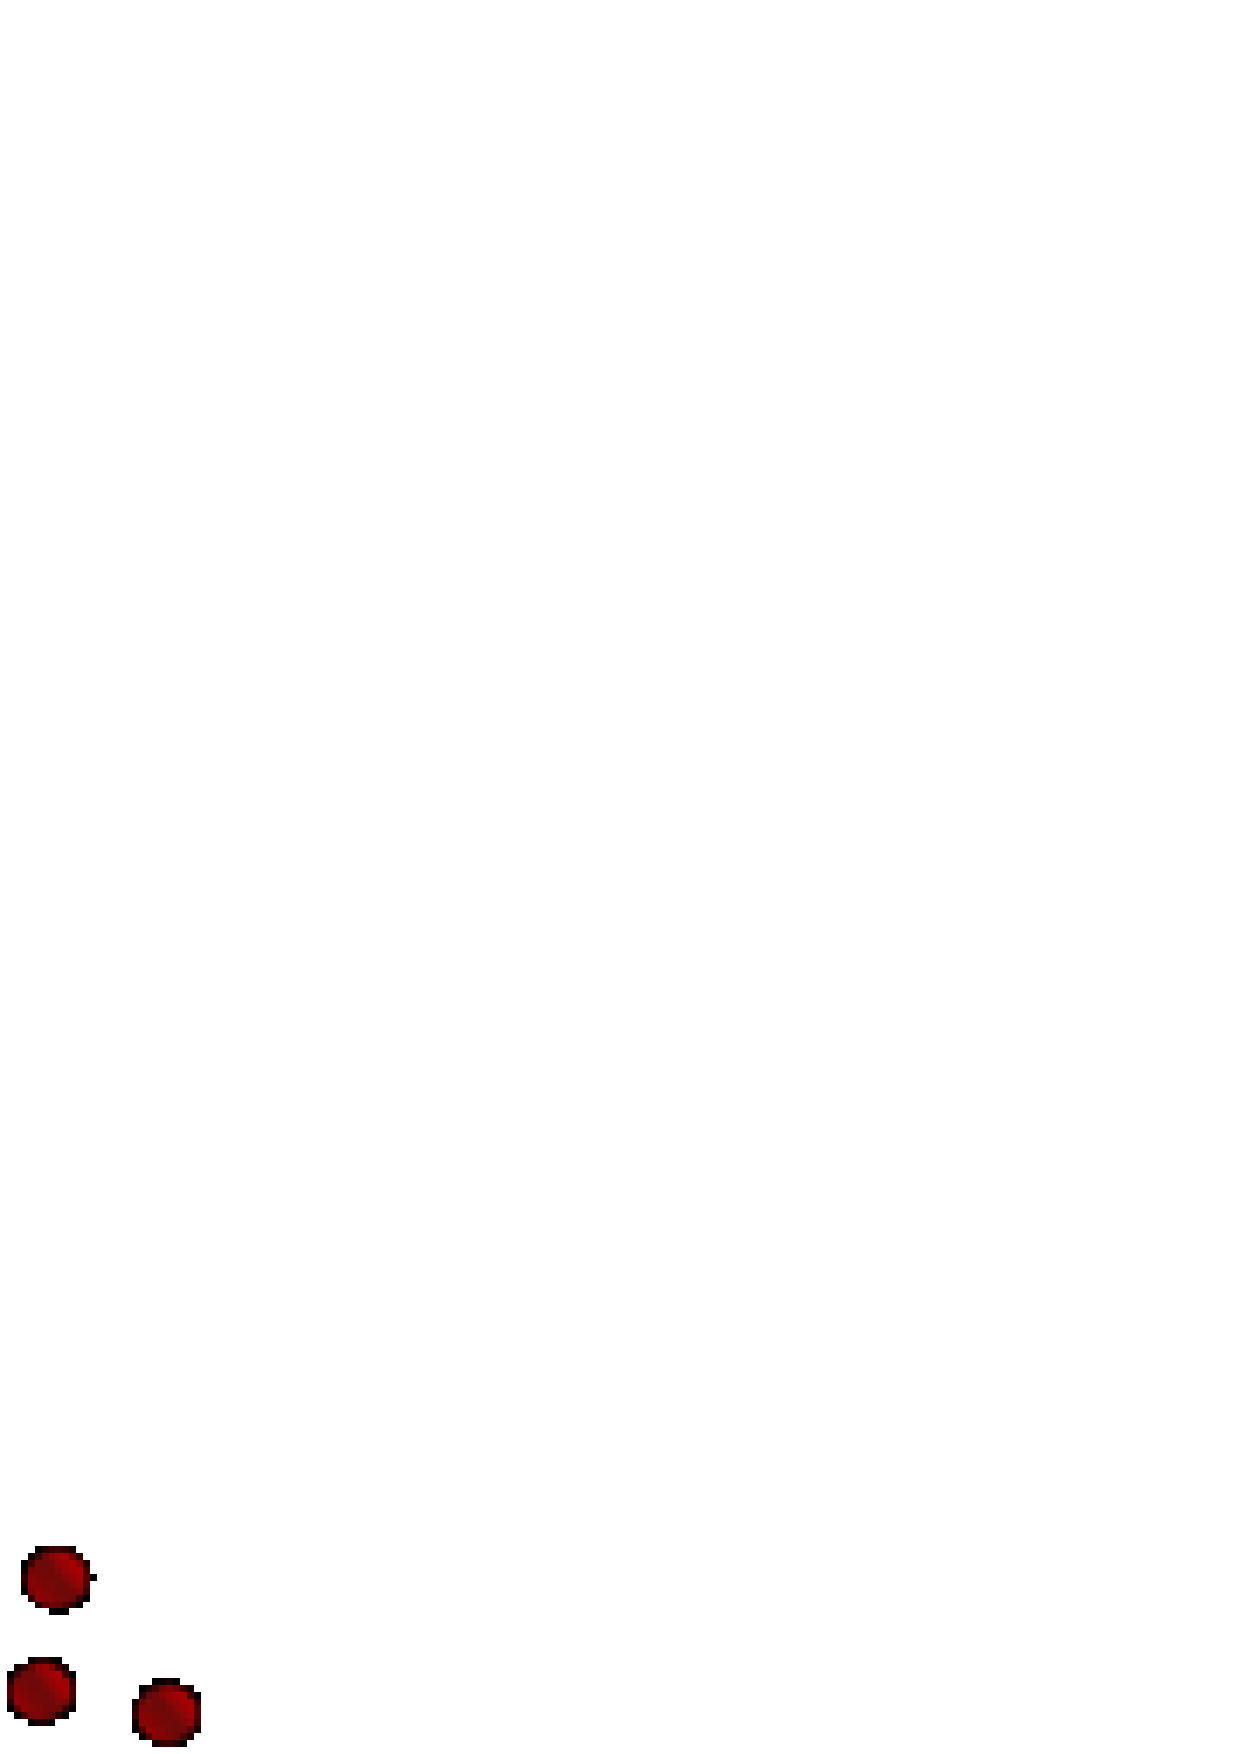
\includegraphics[width=0.7cm]{grass_new_point} & Nouveau Point & Numérise un nouveau point \\
\hline 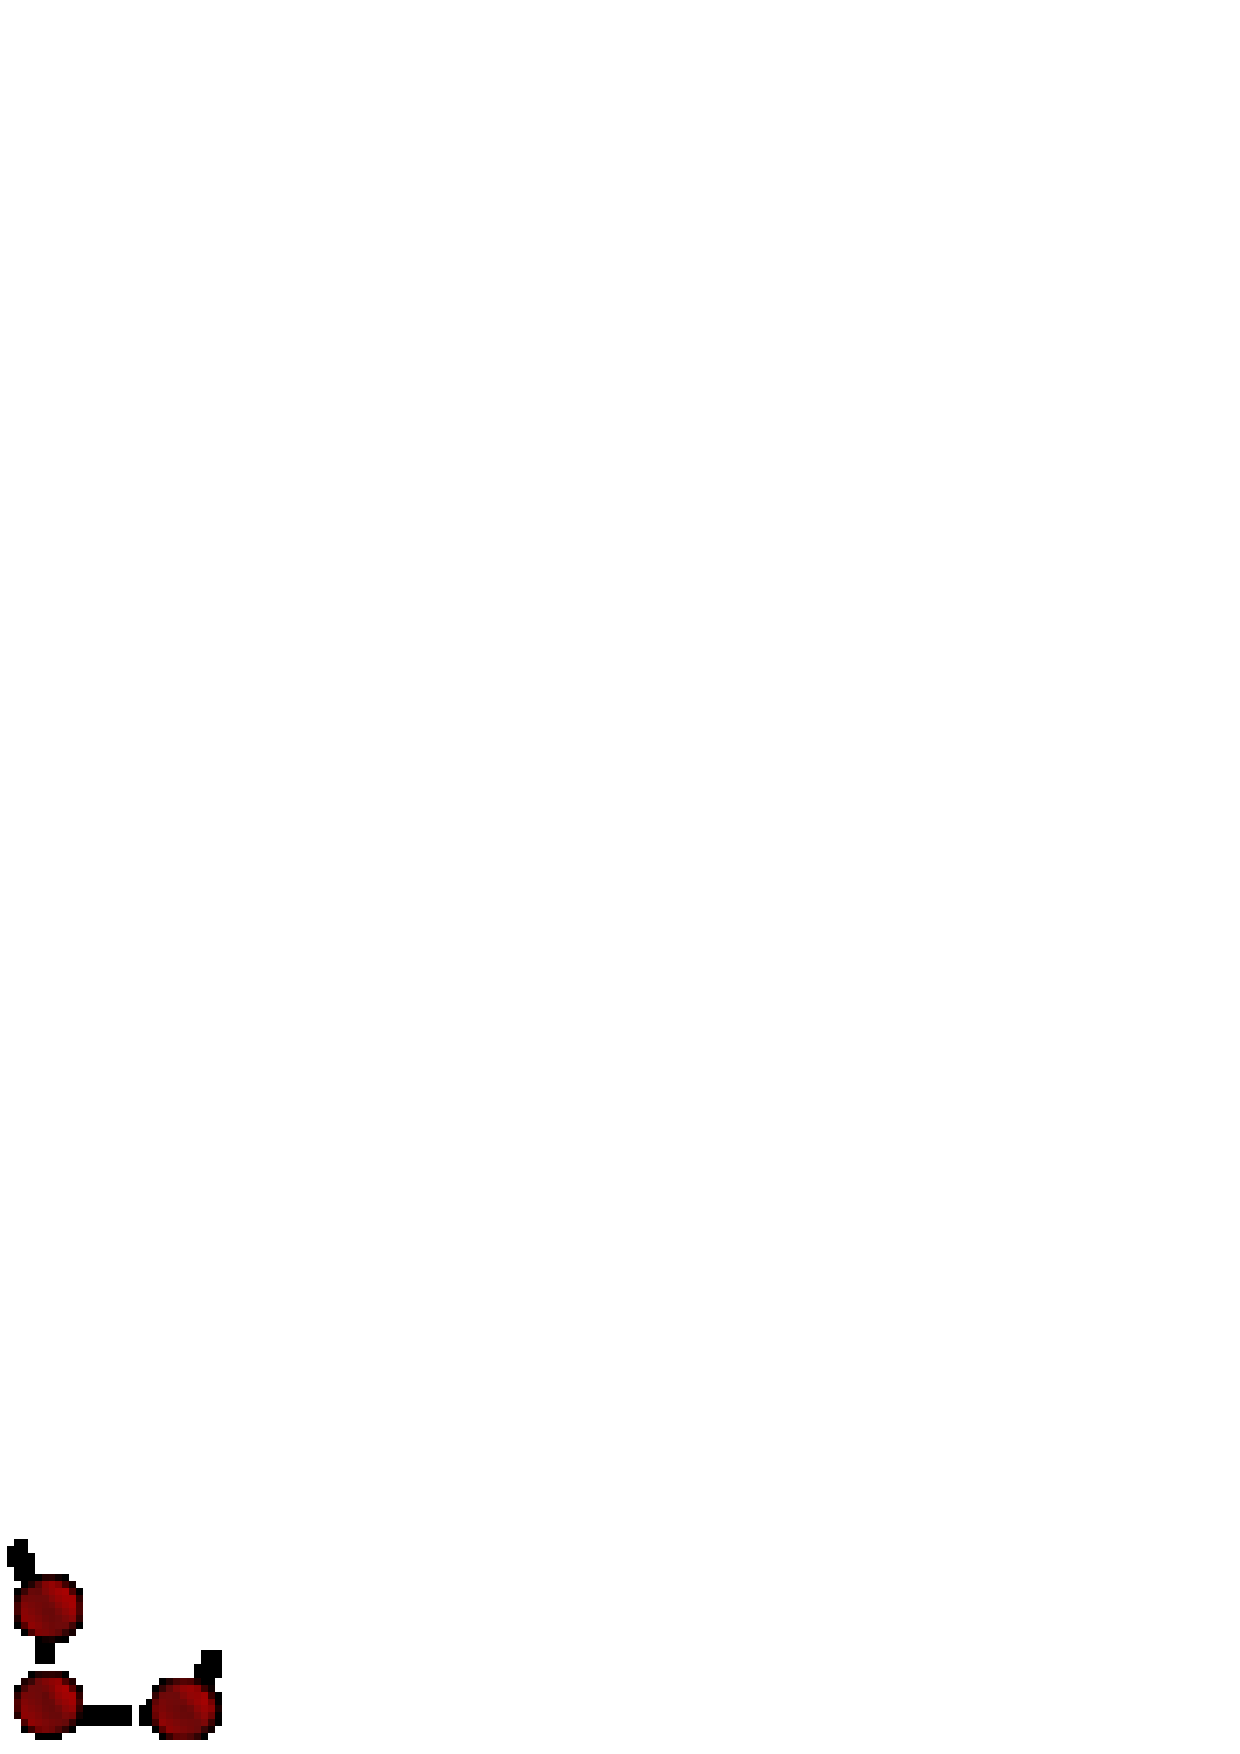
\includegraphics[width=0.7cm]{grass_new_line} & Nouvelle Ligne & Numérise une nouvelle ligne (terminez la numérisation en sélectionnant un nouvel outil) \\
\hline 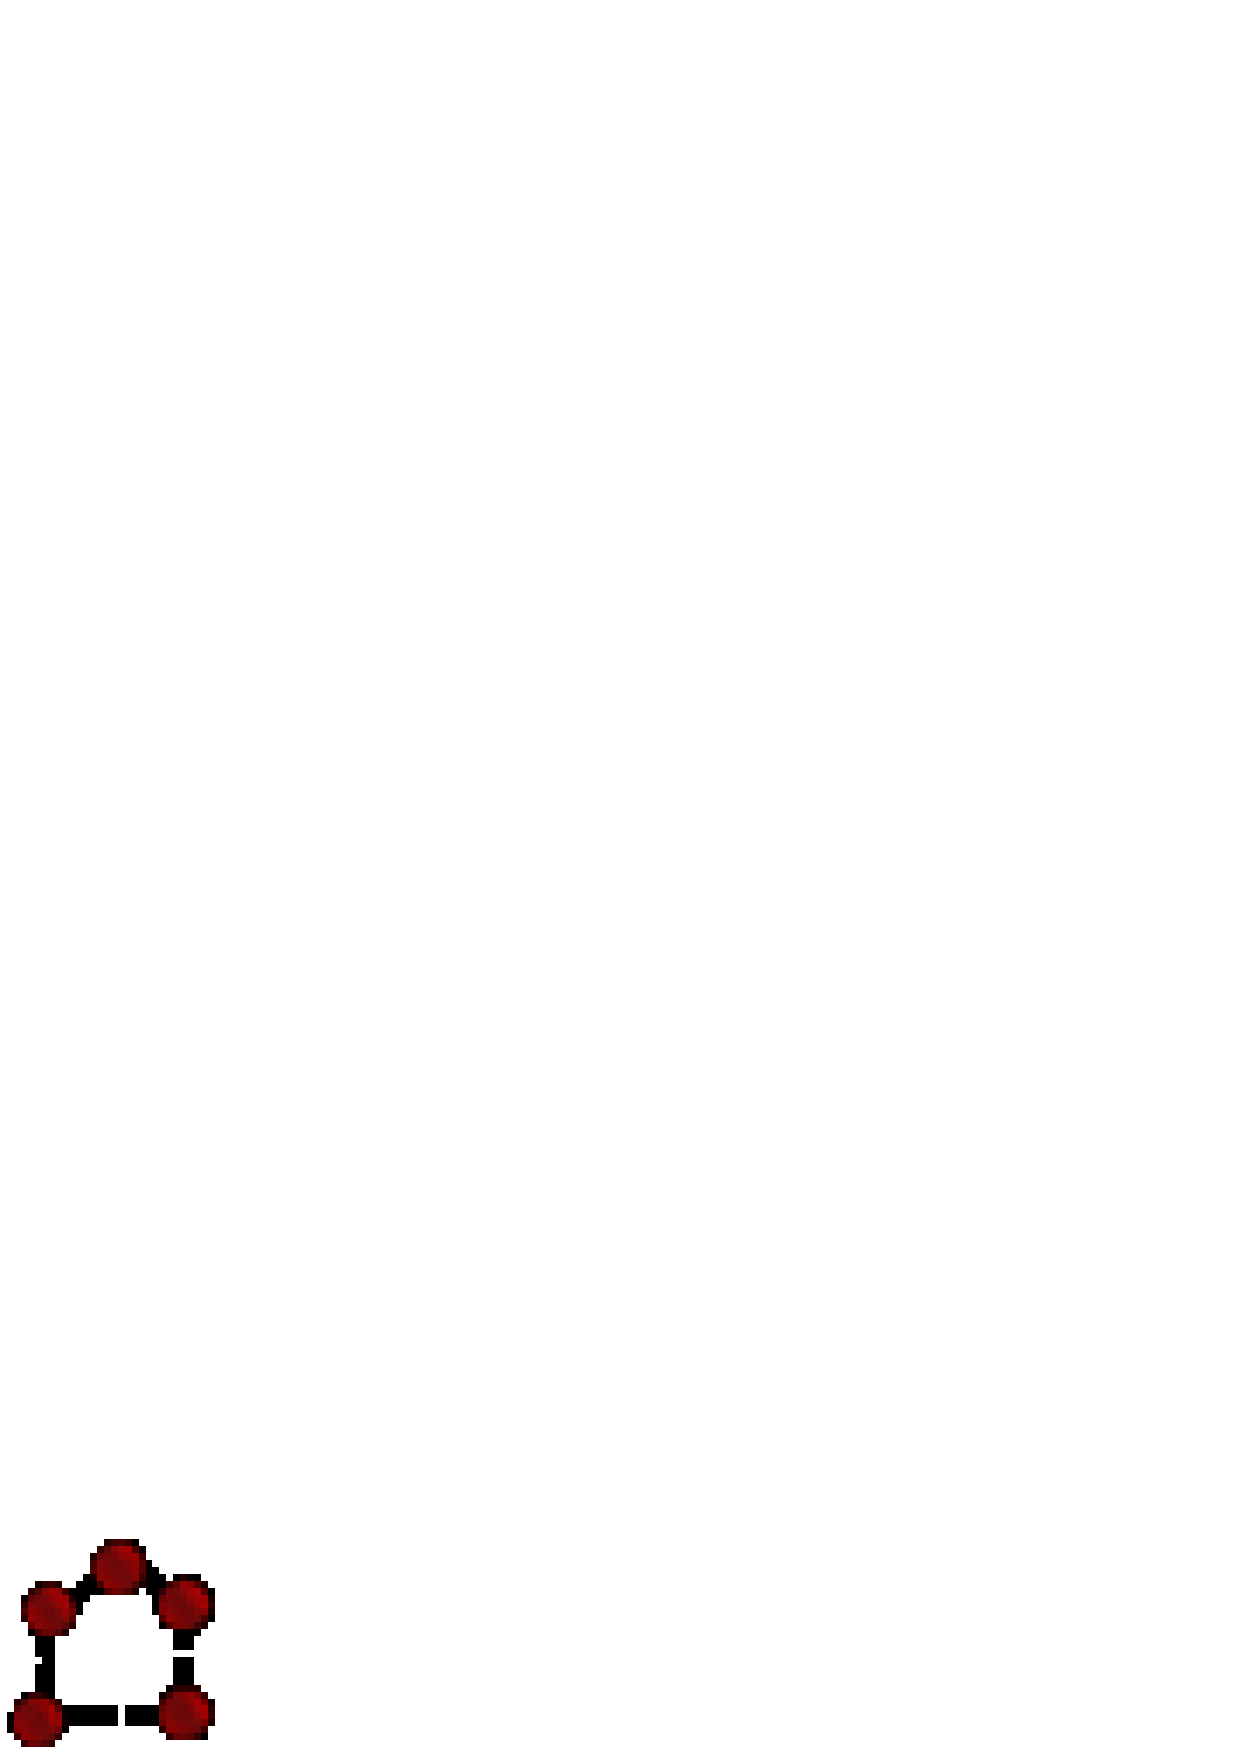
\includegraphics[width=0.7cm]{grass_new_boundary} & Nouveau Contour & Numérise un nouveau contour (terminer la numérisation en sélectionnant un nouvel outil)\\
\hline 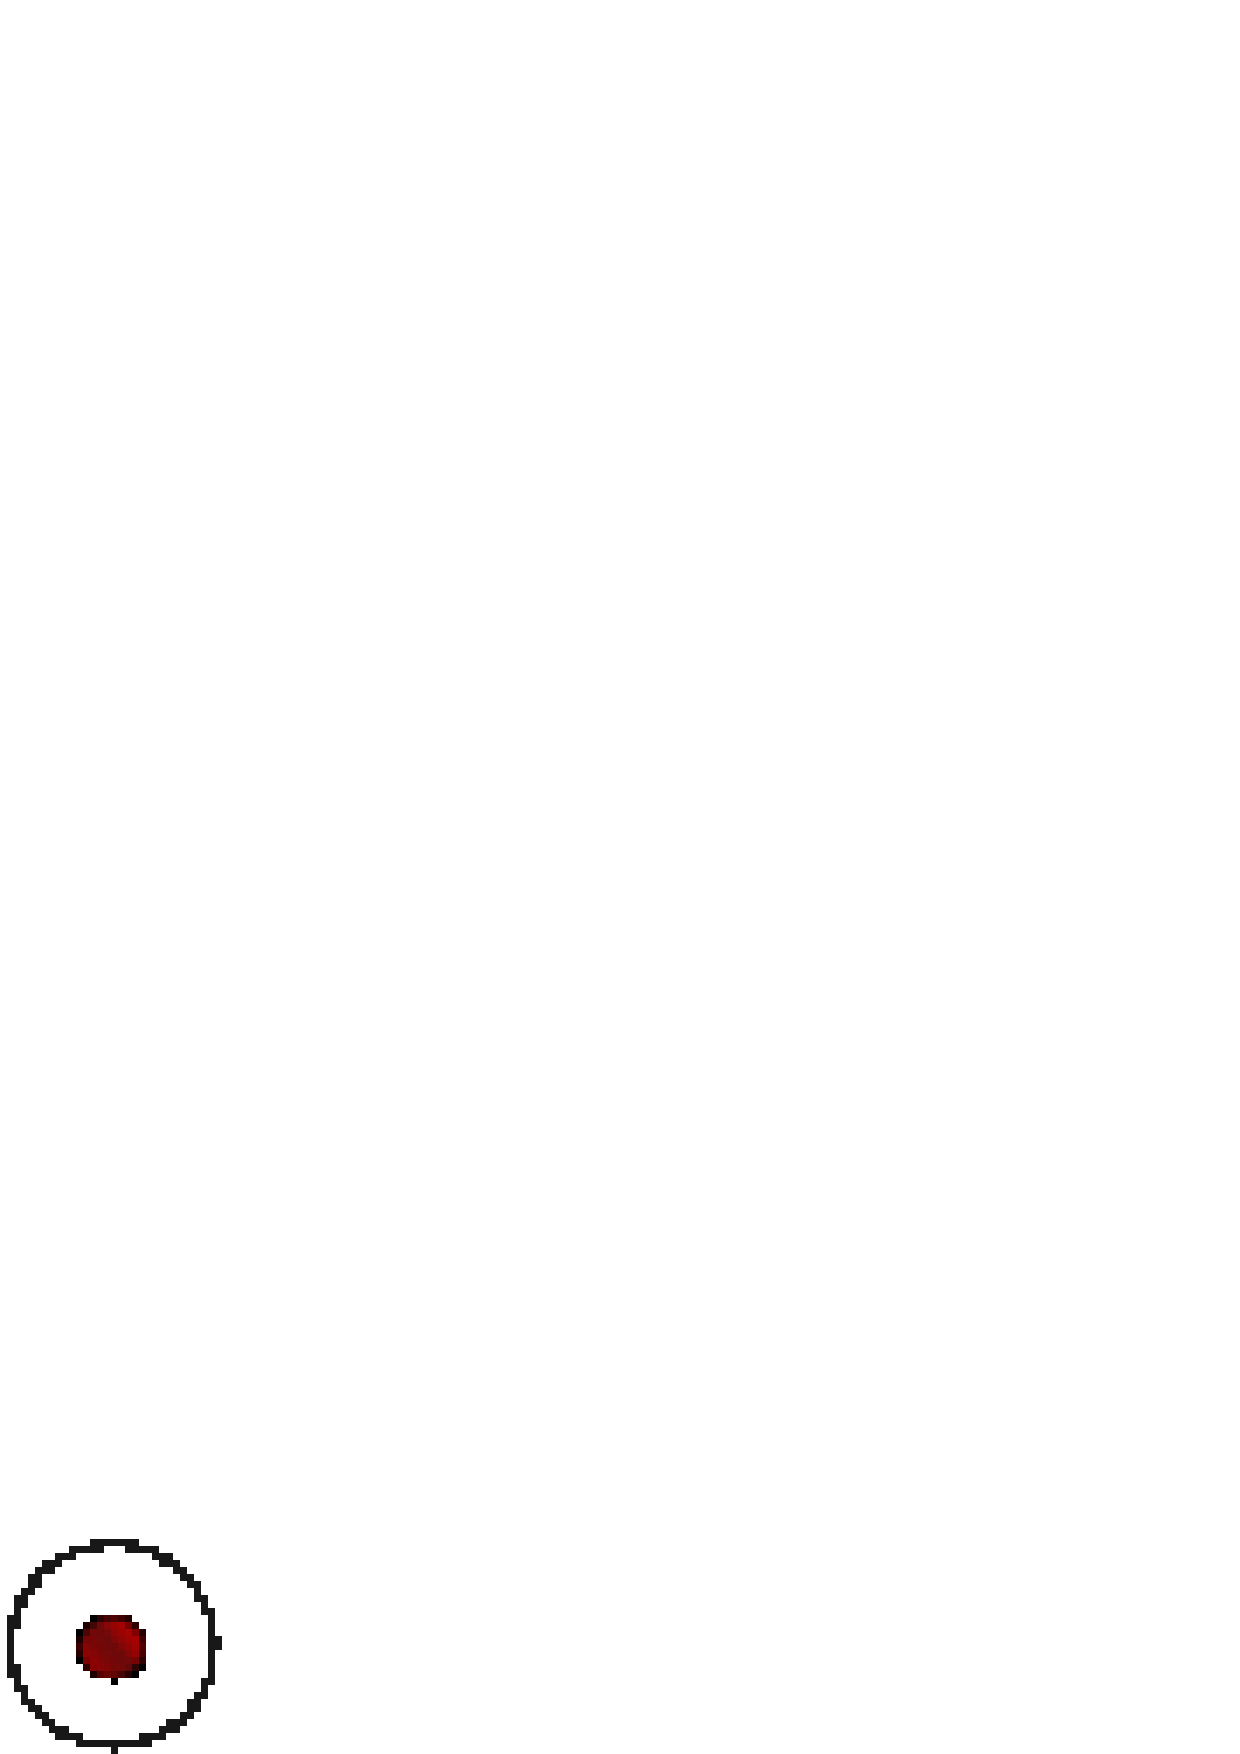
\includegraphics[width=0.7cm]{grass_new_centroid} & Nouveau Centro"ide & Numérise un nouveau centro"ide (emplacement de l'étiquette d'un polygone existant)\\
\hline 
\includegraphics[width=0.7cm]{grass_move_vertex} & Déplacer le sommet & Déplace un sommet d'une ligne ou d'un polygone existant et indique sa nouvelle position\\
\hline 
\includegraphics[width=0.7cm]{grass_add_vertex} & Ajouter un sommet & Ajoute un nouveau sommet à une ligne existante\\
\hline 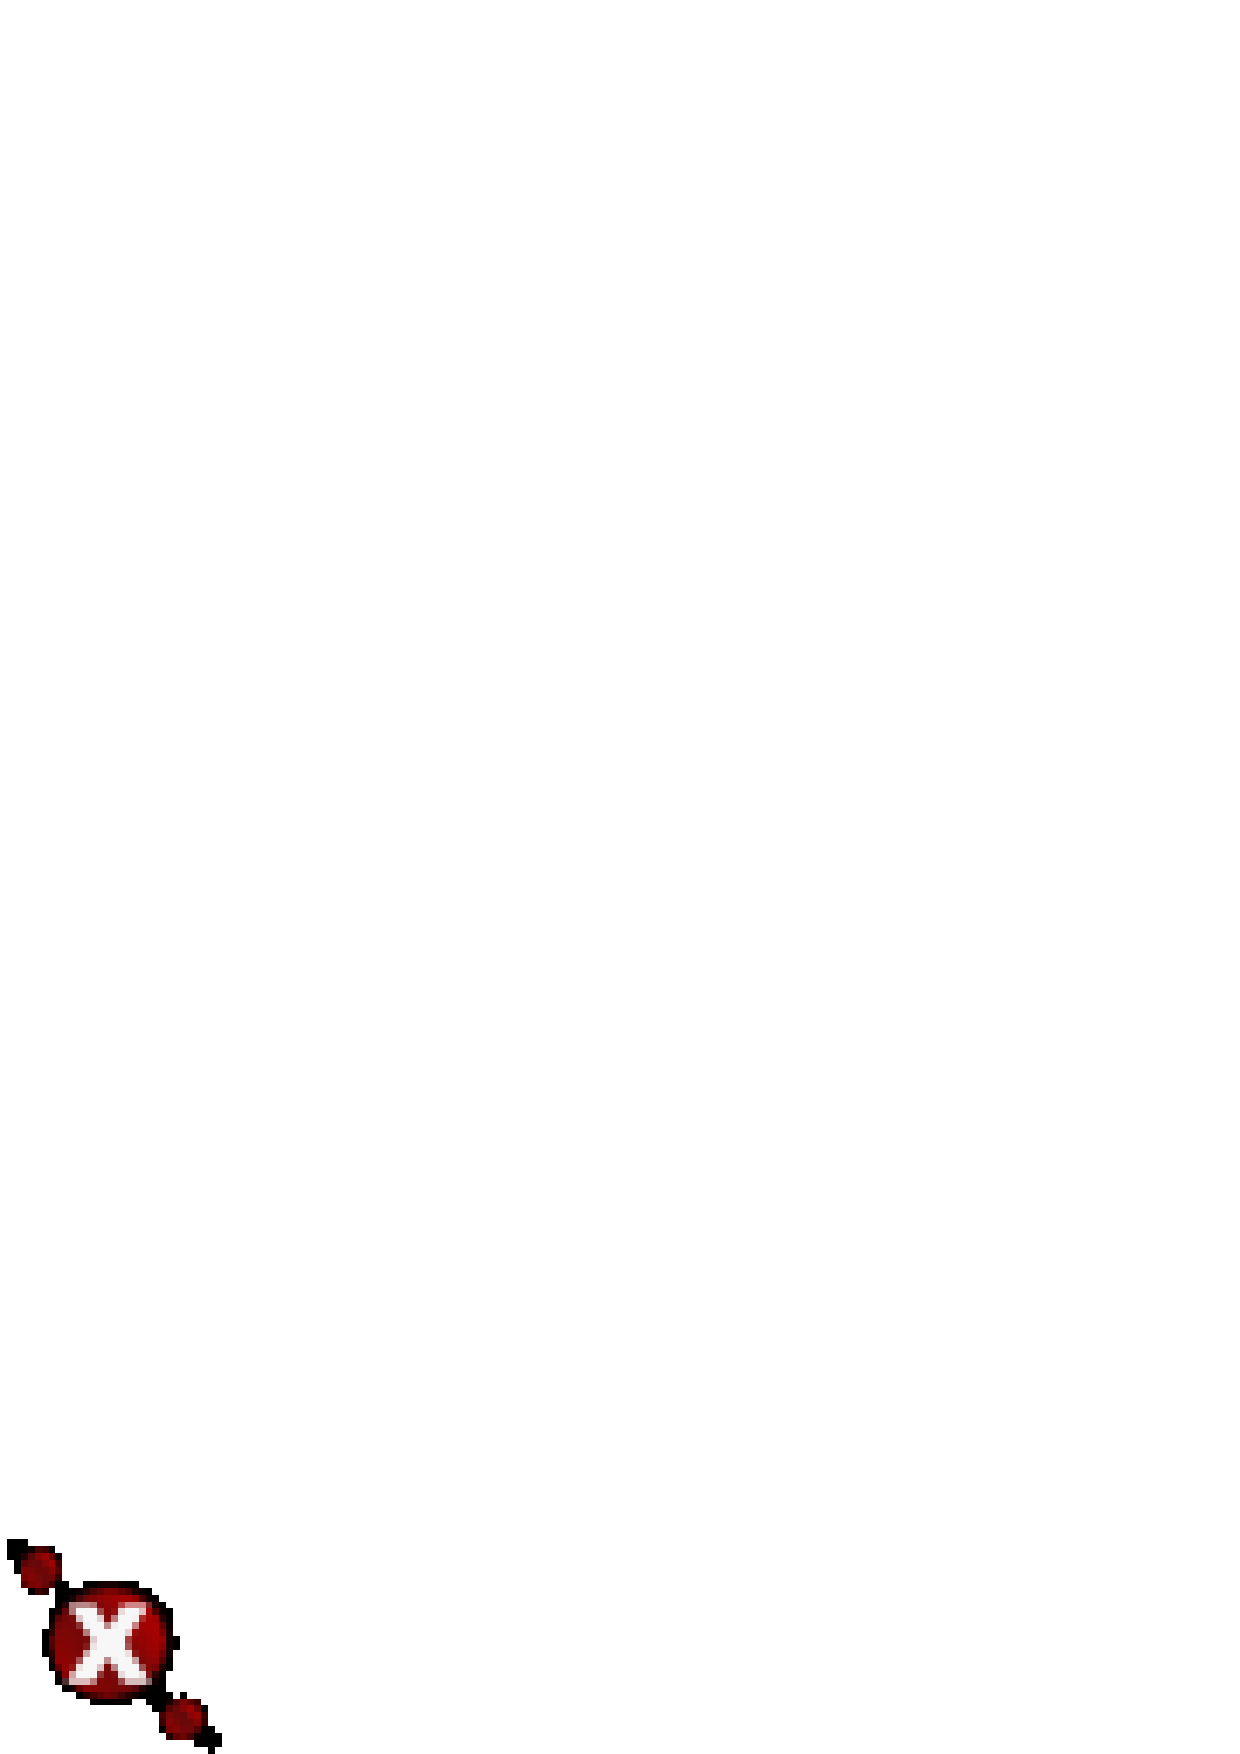
\includegraphics[width=0.7cm]{grass_delete_vertex} & Effacer un sommet & Efface un sommet d'une ligne existante (confirmez le sommet sélectionné avec un autre clic)\\
\hline 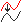
\includegraphics[width=0.7cm]{grass_move_line} & Déplace l'élément & Déplacez la limite, la ligne, le point ou le centro"ide sélectionné puis cliquez sur la nouvelle position\\
\hline 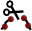
\includegraphics[width=0.7cm]{grass_split_line} & Coupe la ligne & Coupe une ligne existante en deux parties\\
\hline 
\includegraphics[width=0.7cm]{grass_delete_line} & Efface l'élément & Efface une limite, une ligne, un point ou un centro"ide existant (confirmez l'élément sélectionné avec un autre clic)\\
\hline 
\includegraphics[width=0.7cm]{grass_edit_attributes} & Éditer les attributs & Édite les attributs de l'élément sélectionné (notez qu'un seul élément peut représenter plusieurs géométries, voir ci-dessus)\\
\hline 
\includegraphics[width=0.7cm]{grass_close_edit} & Fermer & Ferme la session et sauvegarde l'état actuel (reconstruit la topologie après)\\
\hline
\end{tabular}
\end{table}

%\minisec{Category Tab}\index{GRASS!category settings}
\minisec{Onglet Categorie}\index{GRASS!paramètres de catégorie}
%The \tab{Category} tab allows you to define the way in which the category values will be assigned to a new geometry element.
L'onglet \tab{Categorie} vous permet de définir la manière dont les valeurs du champ category sont assignées au nouvel élément géométrique.

\begin{figure}[h]
 \begin{center}
  %\caption{GRASS Digitizing Category Tab \nixcaption}\label{fig:grass_digitizing_category}
  \caption{Onglet Catégorie d'Édition GRASS \nixcaption}\label{fig:grass_digitizing_category}
  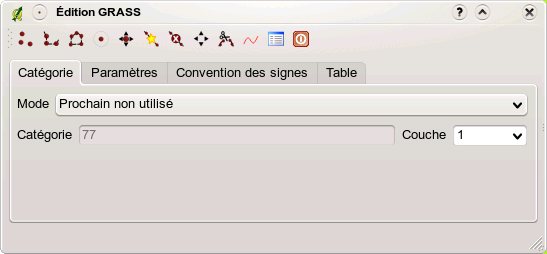
\includegraphics[clip=true,width=10cm]{grass_digitizing_category}
 \end{center}
\end{figure}

\begin{itemize}
%\item \textbf{Mode}: what category value shall be applied to new geometry elements.
\item \textbf{Mode}: quelle catégorie sera appliqué au nouvel élément.
\begin{itemize}
%\item Next not used - apply next not yet used category value to geometry element.
\item Prochain non utilisé - applique la valeur suivante non utilisée du champ category à l'élément géométrique.
%\item Manual entry - manually define the category value for the geometry element in the 'Category'-entry field.
\item Saisie manuelle - saisir manuellement la valeur du champ category pour l'élément géométrique.
%\item No category - Do not apply a category value to the geometry element. This is e.g. used for area boundaries, because the category values are connected via the centroid.
\item Pas de catégorie - ne pas remplir le champ category. C'est par exemple utilisé pour les surfaces car les valeurs de catégorie sont stockées via le centro"ide
\end{itemize}
%\item \textbf{Category} - A number (ID) is attached to each digitized geometry element. It is used to connect each geometry element with its attributes.
\item \textbf{Categorie} - un identifiant (ID) est attaché à chaque objet numérisé. Il est utilisé pour connecter les objets géométriques avec ces attributs.
%\item \textbf{Field (layer)} - Each geometry element can be connected with several attribute tables using different GRASS geometry layers. Default layer number is 1. 
\item \textbf{Couche} - Chaque objet peut être connecté à différentes tables attributaires au travers des différentes sous-couches. Le numéro de sous-couche par défaut est 1.

\end{itemize}

%\begin{Tip}\caption{\textsc{Creating an additional GRASS 'layer' with QGIS}}
\begin{Astuce}\caption{\textsc{Création d'une sous-couche supplémentaire avec QGIS}}
%\qgistip{If you would like to add more layers to your dataset, just add a new number in the 'Field (layer)' entry box and press return. 
%In the Table tab you can create your new table connected to your new layer.
\qgistip{Si vous souhaitez avoir plusieurs sous-couches dans votre couche vecteur, ajouter simplement un nouveau chiffre dans la zone de saisie 'Couche' et appuyez sur entrée. Dans l'onglet Table, vous pouvez créer de nouvelles tables attributaires connectées à votre nouvelle sous-couche.
}
\end{Astuce}

\minisec{Onglet Paramètres}\label{label_settingtab}\index{GRASS!tolérance d'accrochage}

%The \tab{Settings} tab allows you to set the snapping in screen pixels. The threshold defines at what distance new points or line ends are snapped to
%existing nodes. This helps to prevent gaps or dangles between boundaries. The default is set to 10 pixels.
L'onglet \tab{Paramètres} vous permet de définir la tolérance d'accrochage en pixels écran. Le seuil définit à partir de quelle distance les nouveaux points ou les nouvelles lignes sont accrochées automatiquement à des noeuds existants. Cela aide à éviter de créer des trous ou des superpositions entre les contours. La valeur par défaut est fixée à 10 pixels.

\begin{figure}[h]
 \begin{center}
% \caption{GRASS Digitizing Settings Tab \nixcaption}\label{fig:grass_digitizing_settings}
 \caption{Onglet Paramètres d'Édition GRASS \nixcaption}\label{fig:grass_digitizing_settings}
 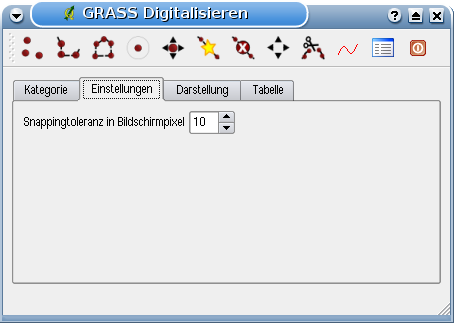
\includegraphics[clip=true,width=8cm]{grass_digitizing_settings}
 \end{center}
\end{figure}

%\minisec{Symbology Tab}\index{GRASS!symbology settings}
\minisec{Onglet Convention des signes}\index{GRASS!convention des signes}

%The \tab{Symbology} tab allows you to view and set symbology and color settings for various geometry types and their topological status (e.g. closed / opened boundary).
L'onglet \tab{Convention des signes} vous permet d'afficher et modifier la symbologie, la couleur des différentes formes géométriques ainsi que leur statut topologique (par exemple : contour ouvert / fermé)

\begin{figure}[h]
 \begin{center}
 %\caption{GRASS Digitizing Symbolog Tab \nixcaption}\label{fig:grass_digitizing_symbology}
 \caption{Onglet Convention des signes d'Édition GRASS \nixcaption}\label{fig:grass_digitizing_symbology}
 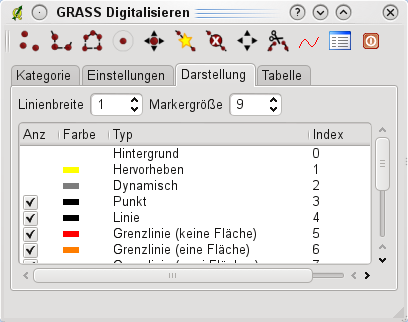
\includegraphics[clip=true,width=8cm]{grass_digitizing_symbology}
 \end{center}
\end{figure}

%\minisec{Table Tab} \index{GRASS!table editing}
\minisec{Onglet Table} \index{GRASS!Éditer une table}
%The \tab{Table} tab provides information about the database table for a given 'layer'. Here you can add new columns to an existing attribute table,
%or create a new database table for a new GRASS vector layer (see Section \ref{sec:creating_new_grass_vectors}).
L'onglet \tab{Table} donne des informations sur la table attributaire d'une sous-couche donnée. C'est ici que vous pouvez ajouter des colonnes à une table attributaire existante ou créer une nouvelle table attributaire pour une nouvelle couche vectorielle GRASS (voir Section \ref{sec:creating_new_grass_vectors}).

\begin{figure}[h]
 \begin{center}
% \caption{GRASS Digitizing Table Tab \nixcaption}\label{fig:grass_digitizing_table}
 \caption{Onglet Table du mode Édition GRASS \nixcaption}\label{fig:grass_digitizing_table}
 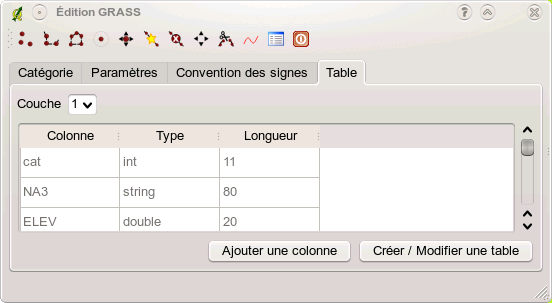
\includegraphics[clip=true,width=10cm]{grass_digitizing_table}
 \end{center}
\end{figure}

\begin{Astuce}\caption{\textsc{Éditer les permissions GRASS}}\index{GRASS!éditer les permissions}
%\qgistip{You must be the owner of the GRASS \filename{MAPSET} you want to edit. It is impossible to edit data layers in a \filename{MAPSET} that is not yours, even if you have write permissions.
\qgistip{Vous devez être propriétaire du \filename{Jeu de données} que vous voulez éditer. Il est impossible de modifier des informations d'un \filename{Jeu de données} qui n'est pas à vous, même si vous avez des droits en écriture.
}
\end{Astuce} 

%\subsection{The GRASS region tool}\label{sec:grass_region}\index{GRASS!region}
\subsection{L'outil région GRASS}\label{sec:grass_region}\index{GRASS!région}

%The region definition (setting a spatial working window) in GRASS is important for working with raster layers. Vector analysis is per default not limited to any defined region definitions. All newly-created rasters will have the spatial extension and resolution of the currently defined GRASS region, regardless of their original extension and resolution. The current GRASS region is stored in the \filename{\$LOCATION/\$MAPSET/WIND} file, and it defines north, south, east and west bounds, number of columns and rows, horizontal and vertical spatial resolution.
La définition d'une région (définir une emprise spatiale de travail) dans GRASS est très importante pour travailler avec des couches rasters. Le travail d'analyse vecteur n'est, par défaut, pas limitée à une région définie. Tous les rasters nouvellement créés auront l'extension spatiale et la résolution de la région GRASS en cours d'utilisation, indépendamment de leur extension et résolution d'origine. La région courante GRASS est stockée dans le fichier \filename{\$LOCATION/\$MAPSET/WIND}, et celui-ci définit les limites Nord, Sud, Est et Ouest, le nombre de lignes et de colonnes ainsi que la résolution spatiale horizontale et verticale.

%It is possible to switch on/off the visualization of the GRASS region in the QGIS canvas using the \toolbtntwo{grass_region}{Display current GRASS region} button. \index{GRASS!region!display}.
Il est possible de d'afficher ou de masquer l'affichage de la région GRASS dans QGIS à l'aide du bouton\toolbtntwo{grass_region}{Afficher la région courante GRASS}. \index{GRASS!région!afficher}.

%With the \toolbtntwo{grass_region_edit}{Edit current GRASS region} icon you can open a dialog to change the current region and the symbology of the GRASS region rectangle in the QGIS canvas. Type in the new region bounds and resolution and click \button{OK}. It also allows to select a new region interactively with your mouse on the QGIS canvas. Therefore click with the left mouse button in the QGIS canvas, open a rectangle, close it using the left mouse button again and click \button{OK}.\index{GRASS!region!editing} The GRASS module \filename{g.region} provide a lot more parameters to define an appropriate region extend and resolution for your raster analysis. You can use these parameters with the GRASS Toolbox, described in Section \ref{subsec:grass_toolbox}.
A l'aide du bouton \toolbtntwo{grass_region_edit}{Éditer la région courante GRASS} vous avez accès à une boîte dialogue qui vous permet de modifier la région courante ainsi que sa symbologie. Entrez les nouvelles limites et résolution et cliquez sur \button{OK}. Cette boîte de dialogue vous permet aussi de définir une nouvelle région interactivement à l'aide de la souris. Pour définir ce rectangle d'emprise, cliquez avec le bouton gauche de la souris et définissez un rectangle que vous terminerez en cliquant de nouveau sur le bouton gauche de la souris et fermez la boîte de dialogue en cliquant sur \button{OK}.\index{GRASS!région!éditer} Le module GRASS \filename{g.region} propose un grand nombre de paramètres pour définir de façon appropriée les limites et la résolution d'une région pour faire de l'analyse raster. Vous pouvez vous servir de ces paramètres dans la boîte à outils GRASS décrite dans la section \ref{subsec:grass_toolbox}.



%\subsection{The GRASS toolbox}\label{subsec:grass_toolbox}\index{GRASS!toolbox}
\subsection{La boîte à outils GRASS}\label{subsec:grass_toolbox}\index{GRASS!boîte à outils} 

%The \toolbtntwo{grass_tools}{Open GRASS Tools} box provides GRASS module functionalities to work with data inside a selected GRASS \filename{LOCATION} and \filename{MAPSET}. To use the GRASS toolbox you need to open a \filename{LOCATION} and \filename{MAPSET} where you have write-permission (usually granted, if you created the \filename{MAPSET}). This is necessary, because new raster or vector layers created during analysis need to be written to the currently selected \filename{LOCATION} and \filename{MAPSET}.
La boîte de dialogue \toolbtntwo{grass_tools}{Ouvrir les outils GRASS} donne accès aux fonctionnalités GRASS qui permettent de travailler dans un \filename{SECTEUR} et sur un \filename{Jeu de Données}. Pour utiliser les outils GRASS, vous devez ouvrir un \filename{SECTEUR} et un \filename{Jeu de Données} sur lequel vous avez des droits d'écriture (que vous avez normalement si vous avez créé le \filename{Jeu de Données}). Cela est nécessaire car les rasters et les vecteurs nouvellement créés lors des analyses doivent être écrits dans le \filename{SECTEUR} et \filename{Jeu de Données} courant.


%\subsubsection{Working with GRASS modules}\index{GRASS!toolbox}
\subsubsection{Travailler avec les modules GRASS}\index{GRASS!boîte à outils} 

\begin{figure}[h]
\centering
%\caption{GRASS Toolbox and searchable Modules List \nixcaption}\label{fig:grass_modules}
%   \subfigure[Modules Tree] {\label{subfig:grass_module_tree}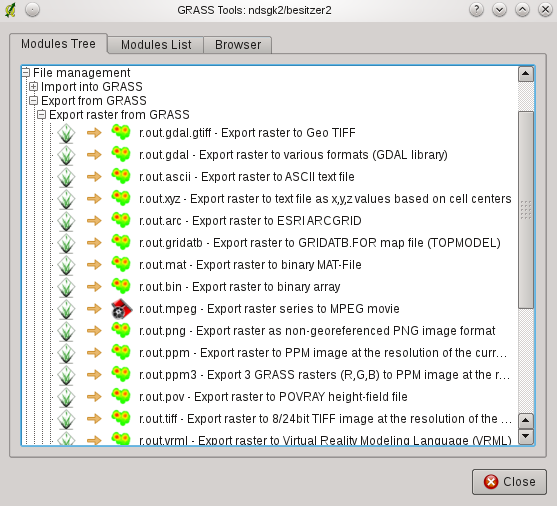
\includegraphics[clip=true, width=0.4\textwidth]{grass_toolbox_moduletree}}\goodgap
%   \subfigure[Searchable Modules List] {\label{subfig:grass_module_list}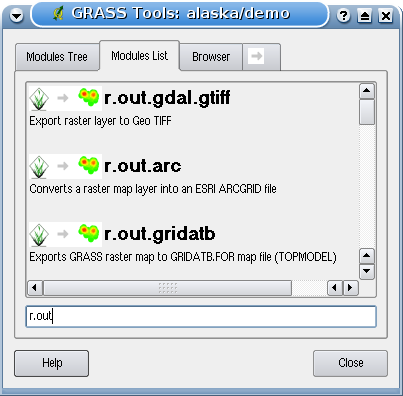
\includegraphics[clip=true, width=0.4\textwidth]{grass_toolbox_modulelist}}
\caption{Outils GRASS et Liste des Modules \nixcaption}\label{fig:grass_modules}
   \subfigure[Arborescence des modules] {\label{subfig:grass_module_tree}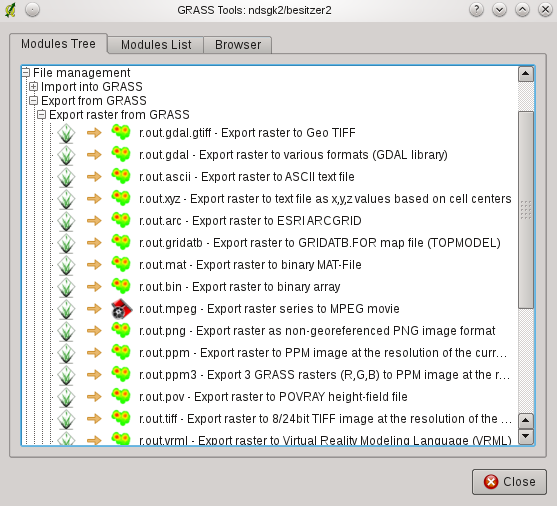
\includegraphics[clip=true, width=0.4\textwidth]{grass_toolbox_moduletree}}\goodgap
   \subfigure[Liste des modules avec possibilité de recherche] {\label{subfig:grass_module_list}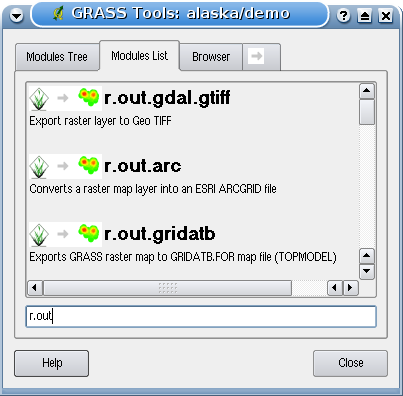
\includegraphics[clip=true, width=0.4\textwidth]{grass_toolbox_modulelist}}
\end{figure}

%The GRASS Shell inside the GRASS Toolbox provides access to almost all (more than 300) GRASS modules in command line modus. To offer a more user friendly working environment, about 200 of the available GRASS modules and functionalities are also provided by graphical dialogs. These dialogs are  grouped in thematic blocks, but are searchable as well. You find a complete list of GRASS modules available in QGIS version \CURRENT in appendix \ref{appdx_grass_toolbox_modules}. It is also possible to customize the GRASS Toolbox content. It is described in Section \ref{sec:toolbox-customizing}.
L'invite de commande de la boîte à outils GRASS vous donne accès à pratiquement tous les modules GRASS (près de 300) en ligne de commande. Afin d'offrir un environnement de travail plus agréable, environ 200 d'entre eux sont fournis avec une boîte de dialogue. Ces boîtes de dialogue sont groupées par thèmes mais sont aussi accessibles par une recherche libre. Vous trouverez une liste complète des modules GRASS disponibles dans QGIS \CURRENT dans l'annexe \ref{appdx_grass_toolbox_modules}. Il est aussi possible de personnaliser le contenu de la boîte à outils GRASS. Ceci est décrit dans la section \ref{sec:toolbox-customizing}.

%As shown in Figure \ref{fig:grass_modules}, you can look for the appropriate GRASS module using the thematically grouped \tab{Modules Tree} or the  searchable \tab{Modules List} tab. 
Comme indiqué sur la figure \ref{fig:grass_modules}, vous pouvez chercher le module GRASS approprié en utilisant l'onglet \tab{Arborescence des modules} ou en utilisant l'onglet \tab{Liste des Modules} pour faire une recherche.

%Clicking on a grapical module icon a new tab will be added to the toolbox dialog providing three new sub-tabs \tab{Options}, \tab{Output} and 
%\tab{Manual}. In Figure \ref{fig:grass_module_dialog} you see an example for the GRASS module \filename{v.buffer}.
Lorsque vous cliquez sur un module, un nouvel onglet apparaît proposant trois sous-onglets \tab{Options}, \tab{Rendu} et \tab{Manuel}. Sur la figure \ref{fig:grass_module_dialog}, vous voyez un exemple pour le module GRASS \filename{v.buffer}.

\begin{figure}[h]
\centering
%\caption{GRASS Toolbox Module Dialogs \nixcaption}\label{fig:grass_module_dialog}
%   \subfigure[Module Options] {\label{subfig:grass_module_option}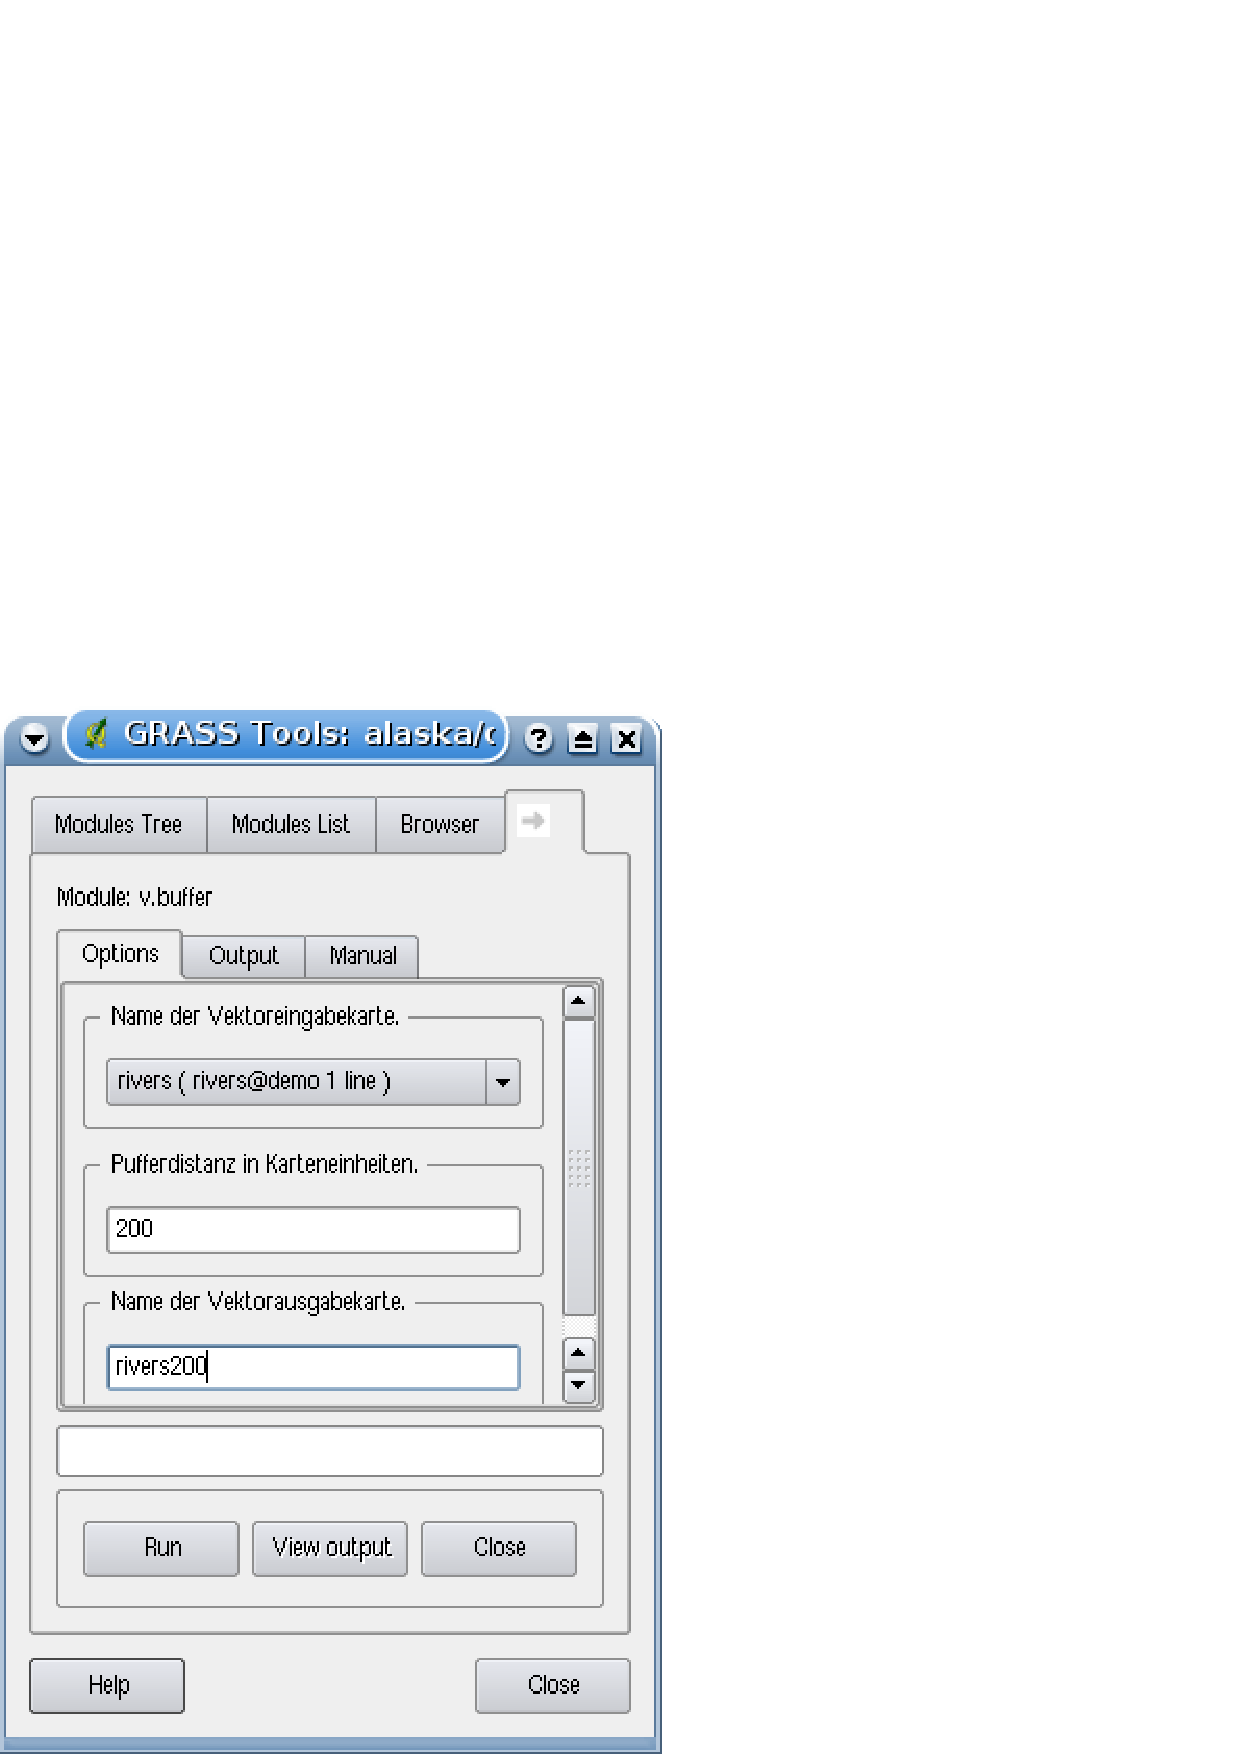
\includegraphics[clip=true, width=0.3\textwidth]{grass_module_option}}\goodgap
%   \subfigure[Modules Output] {\label{subfig:grass_module_output}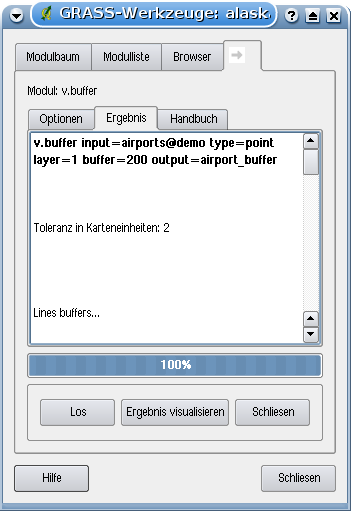
\includegraphics[clip=true, width=0.3\textwidth]{grass_module_output}}\goodgap
%   \subfigure[Module Manual] {\label{subfig:grass_module_manual}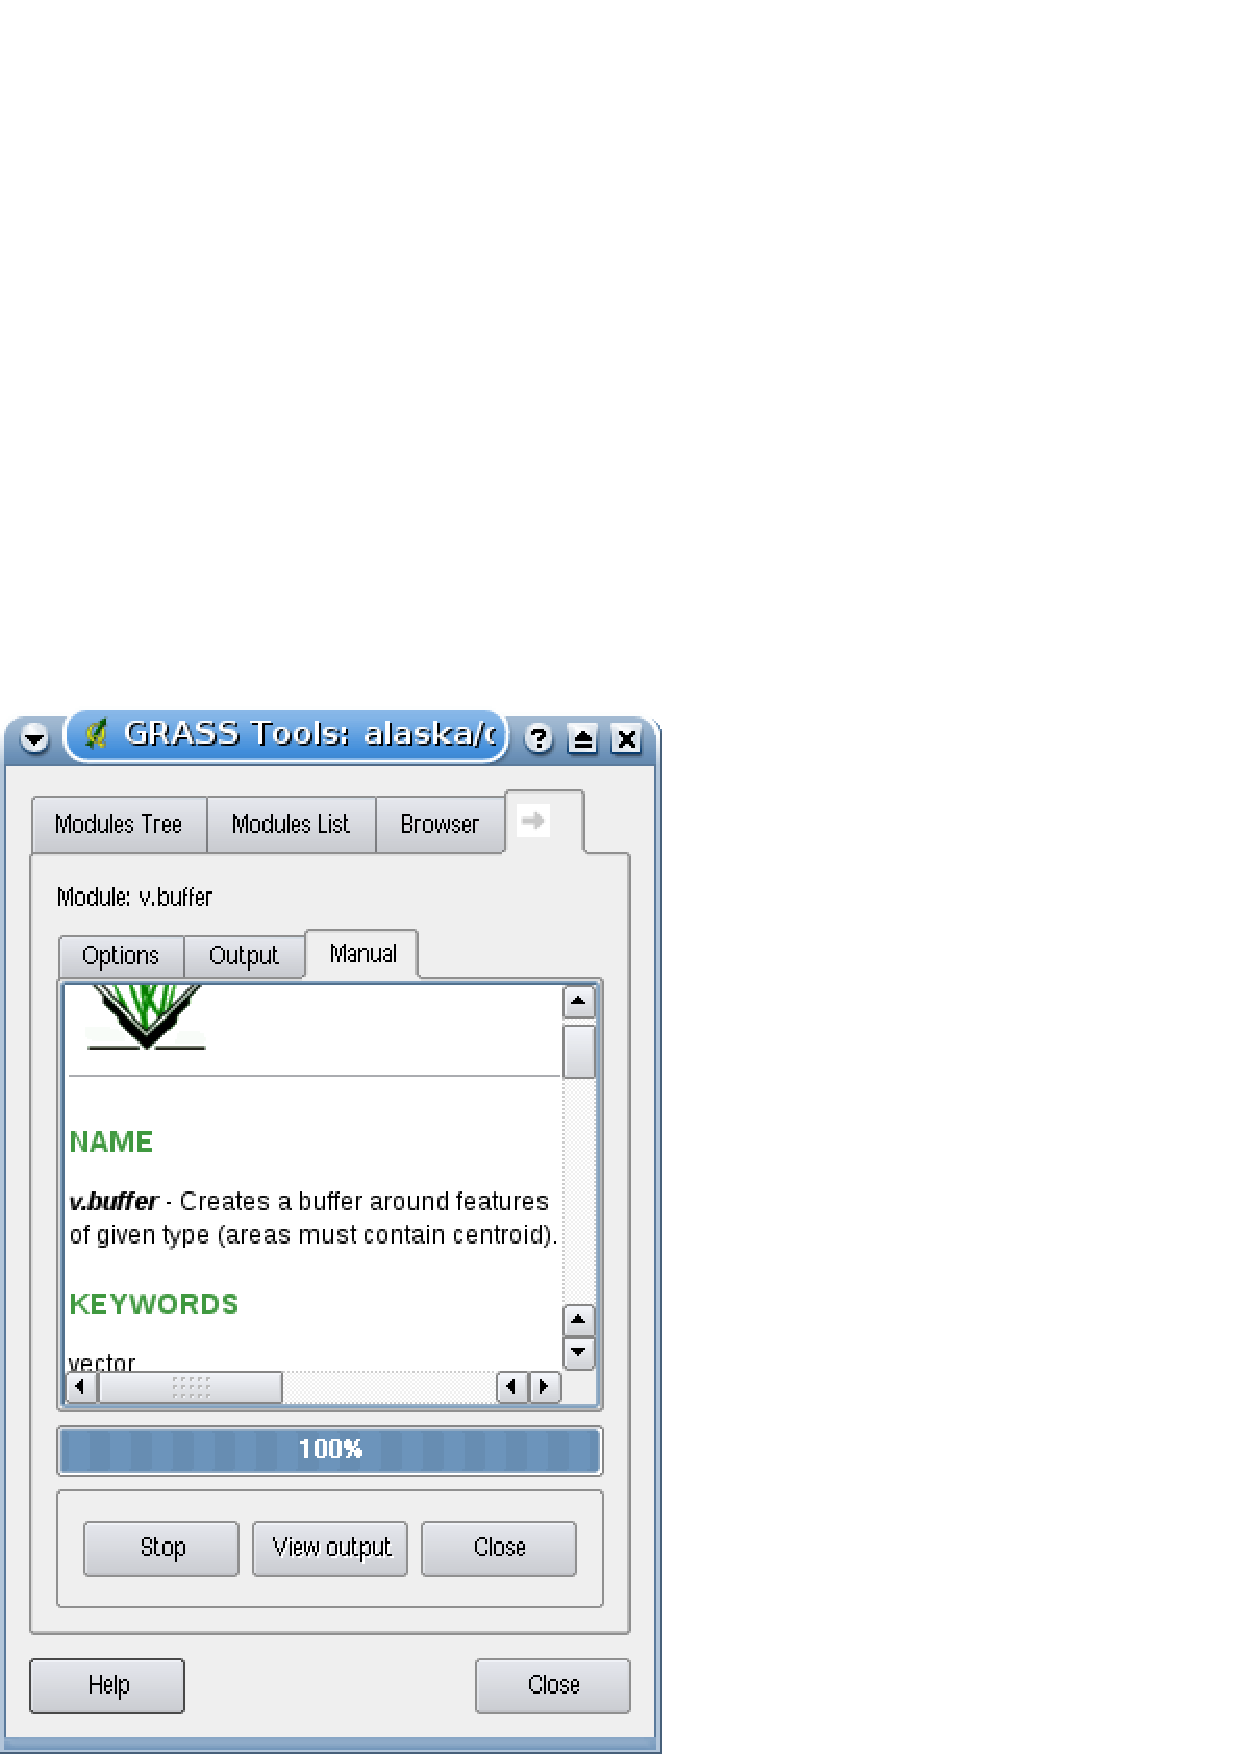
\includegraphics[clip=true, width=0.3\textwidth]{grass_module_manual}}
\caption{Boîte de dialogue d'un module issue des outils GRASS \nixcaption}\label{fig:grass_module_dialog}
   \subfigure[Options du module] {\label{subfig:grass_module_option}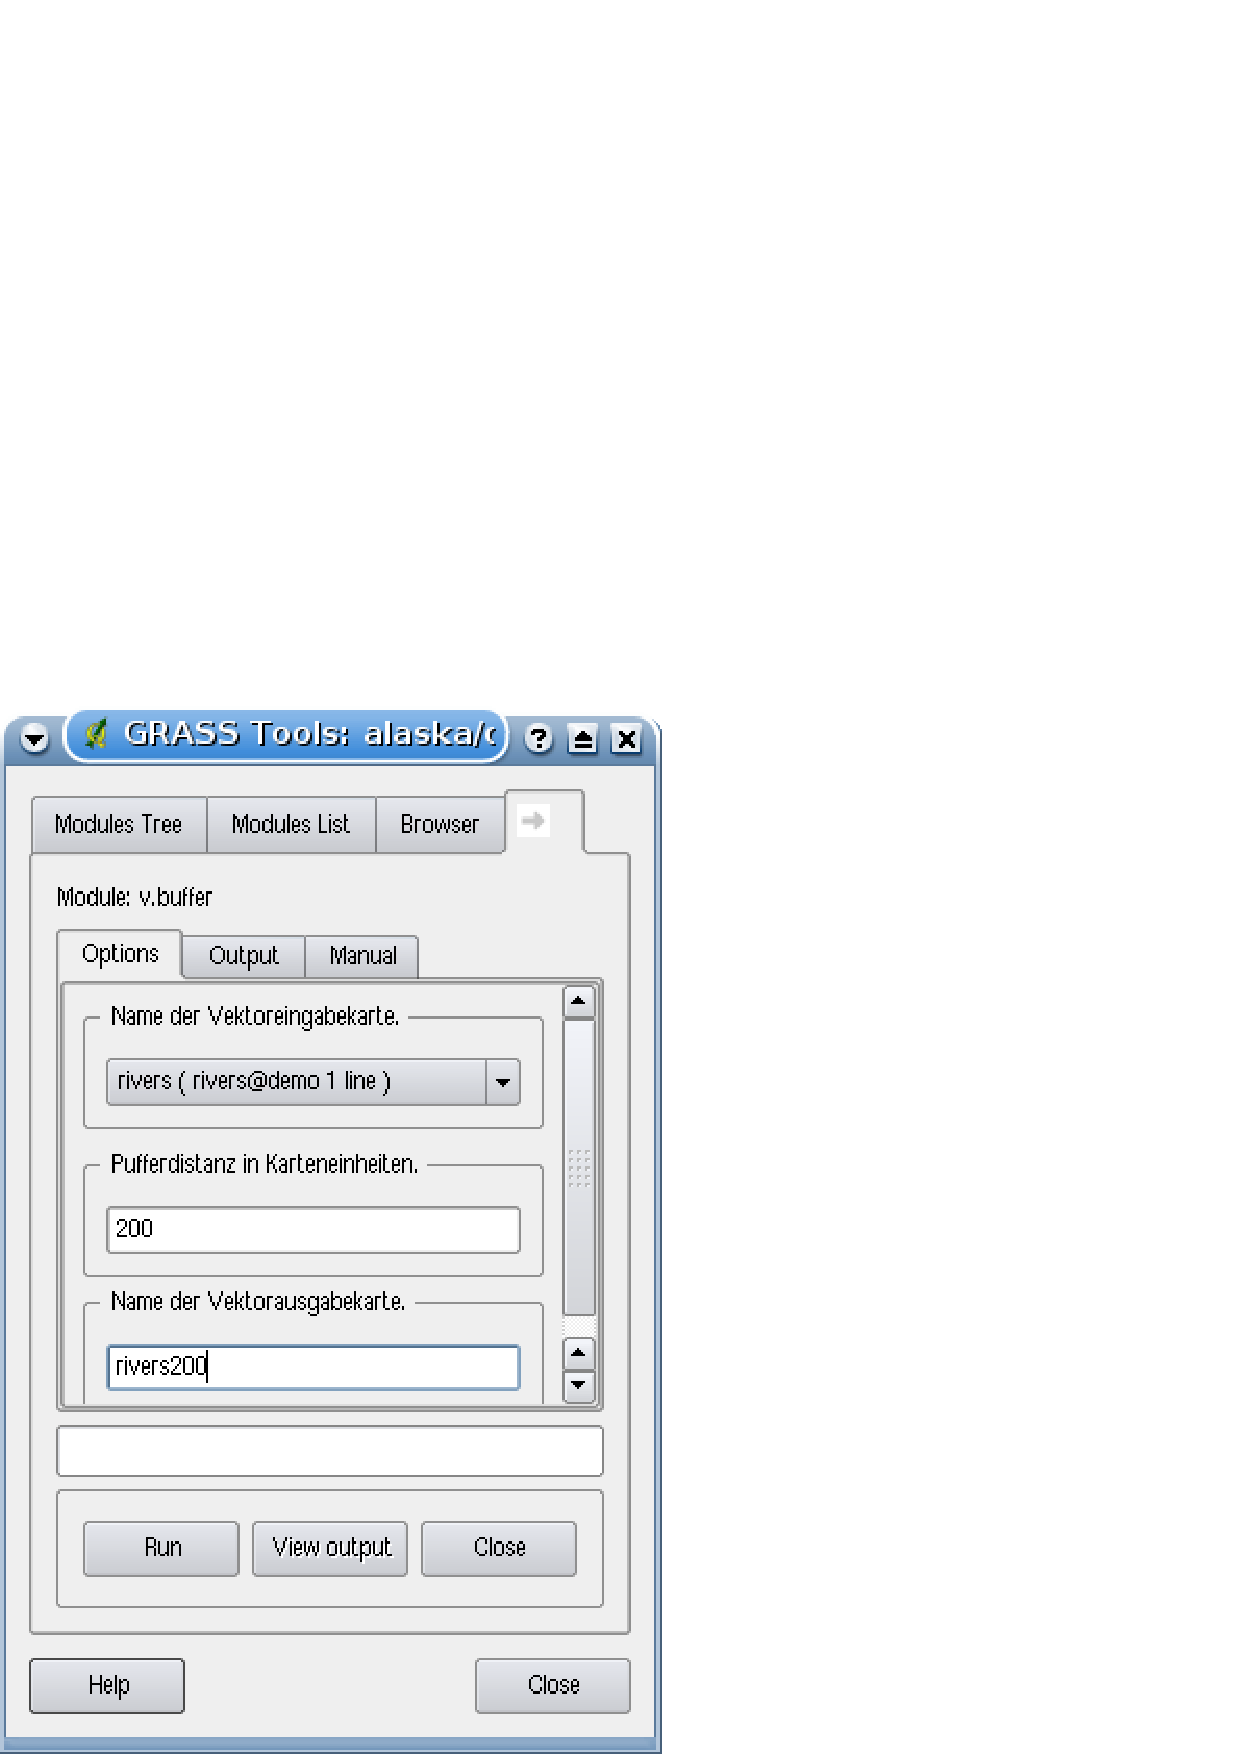
\includegraphics[clip=true, width=0.3\textwidth]{grass_module_option}}\goodgap
   \subfigure[Rendu du module] {\label{subfig:grass_module_output}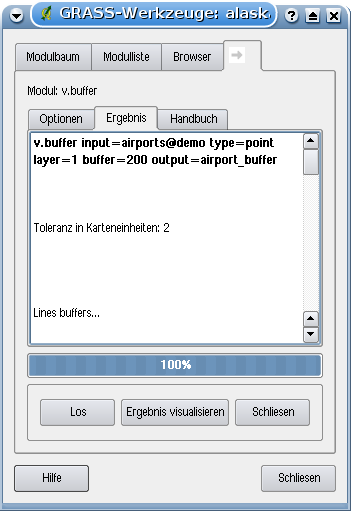
\includegraphics[clip=true, width=0.3\textwidth]{grass_module_output}}\goodgap
   \subfigure[Aide sur le module] {\label{subfig:grass_module_manual}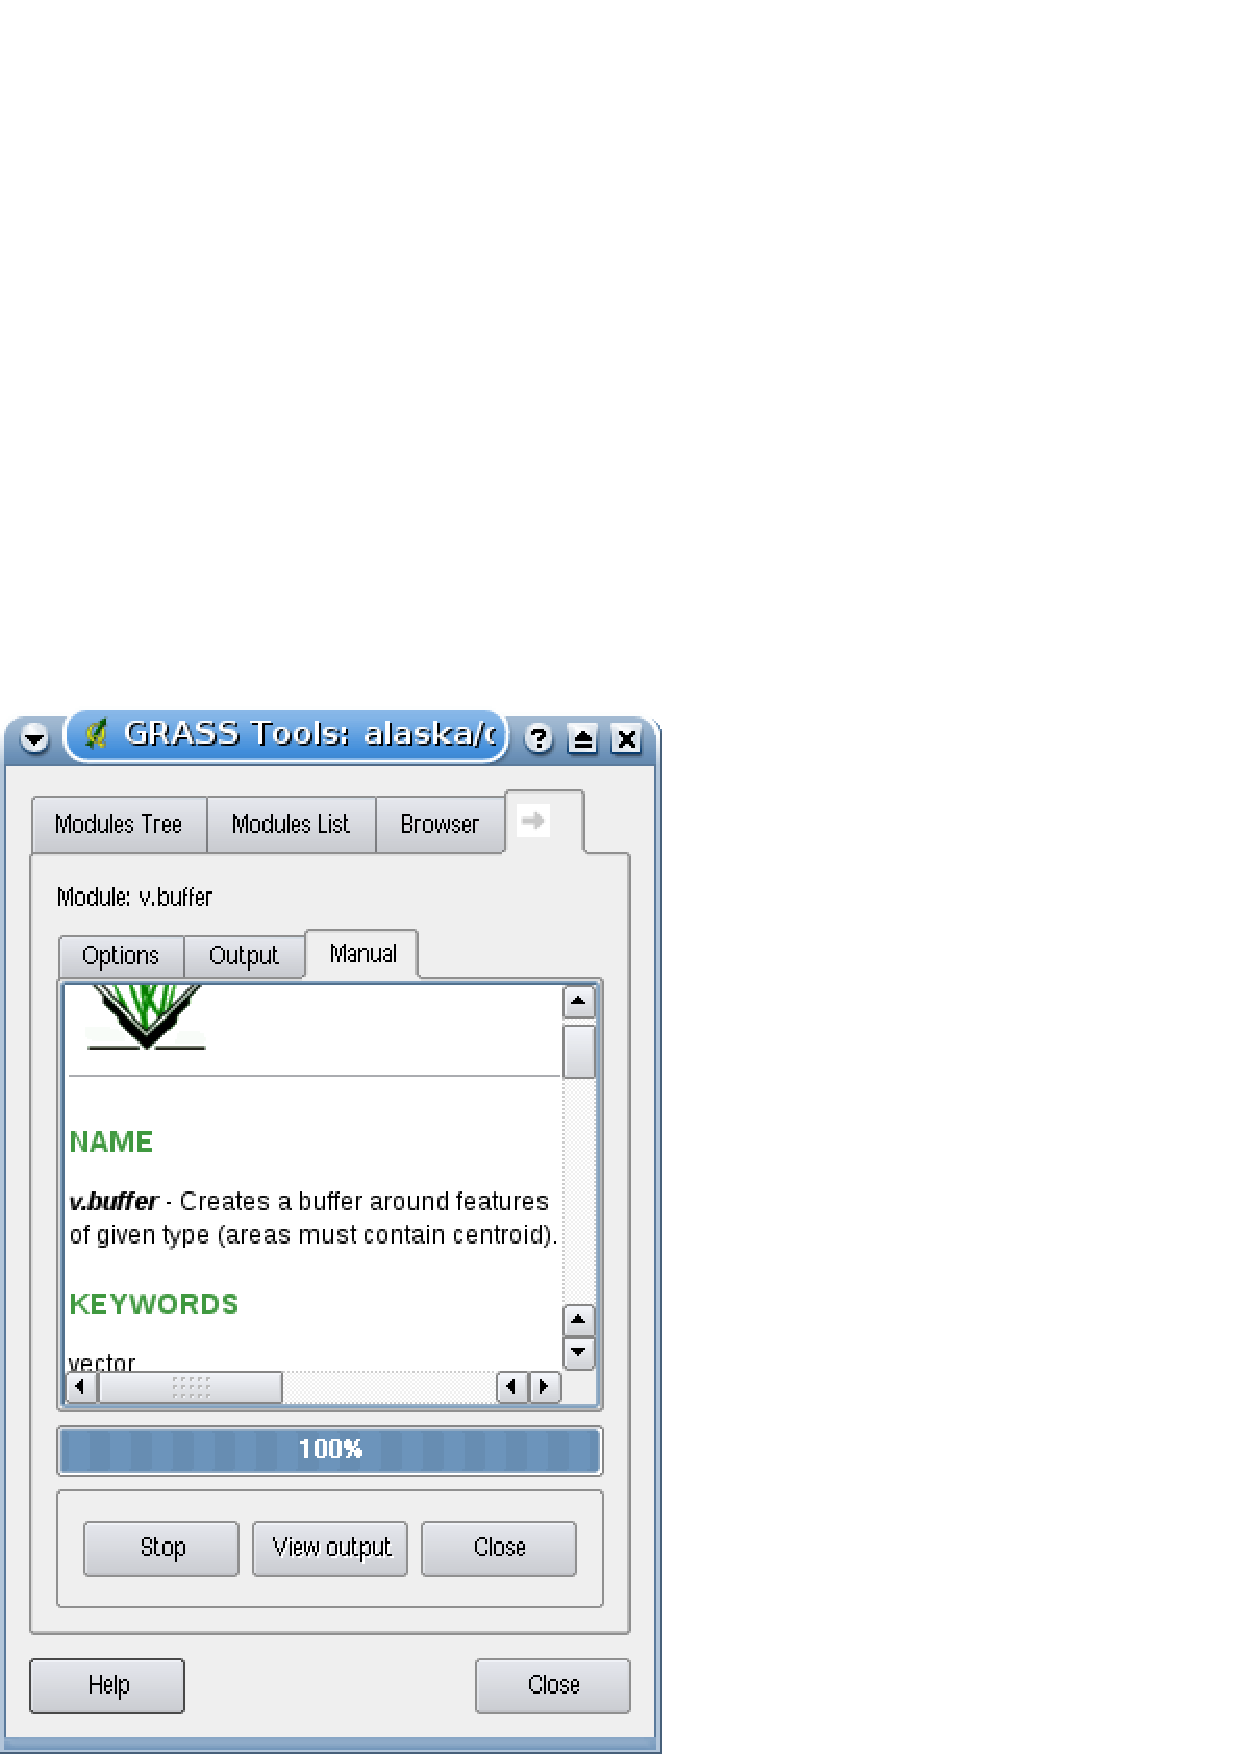
\includegraphics[clip=true, width=0.3\textwidth]{grass_module_manual}}
\end{figure}

\minisec{Options}

%The \tab{Options} tab provides a simplified module dialog where you can usually select a raster or vector layer visualized in the QGIS canvas and 
%enter further module specific parameters to run the module. The provided module parameters are often not complete to keep the dialog clear. If you want to use further module parameters and flags, you need to start the GRASS Shell and run the module in the command line.
L'onglet \tab{Options} propose une interface simplifiée où vous pouvez sélectionner un raster ou un vecteur en cours de visualisation dans QGIS et
saisir les paramètres spécifiques au module avant de le lancer. Tous les paramètres du module ne sont généralement pas fournis afin de simplifier
les boîtes de dialogue. Pour utiliser des paramètres que ne se trouvent pas dans la boîte de dialogue, vous devez utiliser l'invite de commande
et lancer les modules en lignes de commande.

%\minisec{Output}
\minisec{Rendu}

%The \tab{Output} tab provides information about the output status of the module. When you click the \button{Run} button, the module switches to the 
%\tab{Output} tab and you see information about the analysis process. If all works well, you will finally see a \usertext{Successfully finished} message.
L'onglet \tab{Rendu} fournit des informations sur l'état de sortie du module. Quand vous cliquez sur le bouton \button{Lancer}, le module passe sur l'onglet \tab{Rendu} et vous voyez les informations sur le processus en cours. Si tout se passe bien, vous verrez finalement le message \usertext{Terminé avec succès}.
%\minisec{Manual}
\minisec{Manuel}

%The \tab{Manual} tab shows the HTML help page of the GRASS module. You can use it to check further module parameters and flags or to get a deeper 
%knowledge about the purpose of the module. At the end of each module manual page you see further links to the \filename{Main Help index}, the 
%\filename{Thematic index} and the \filename{Full index}. These links provide the same information as if you use the module \filename{g.manual}.
L'onglet \tab{Manuel} montre la page HTML d'aide du module. Vous pouvez vous en servir pour voir les autres paramètres du modules et pour avoir une
connaissance plus approfondie de l'objet du module. A la fin de chaque page d'aide d'un module, vous avez des liens vers \filename{Main Help index},
\filename{Thematic index} et \filename{Full index}. Ces liens vous donnent les mêmes informations que si vous utilisiez \filename{g.manual}.

%\begin{Astuce}\caption{\textsc{Display results immediately}}\index{GRASS!display results}
\begin{Astuce}\caption{\textsc{Afficher les résultats immédiatement}}\index{GRASS!afficher les résultats}
%\qgistip{If you want to display your calculation results immediately in your map canvas, you can use the 'View Output' button at the bottom of the  module tab.
\qgistip{Si vous voulez voir immédiatement dans votre fenêtre carte le résultat du module, vous pouvez utiliser le bouton 'Vue' au bas de l'onglet du module.
}
\end{Astuce} 

%\subsubsection{Working with the GRASS LOCATION browser} \index{GRASS!toolbox!Browser}
\subsubsection{Travailler avec le navigateur GRASS} \index{GRASS!boîte à outils!navigateur}

%Another useful feature inside the GRASS Toolbox is the GRASS \filename{LOCATION} browser. In Figure~\ref{fig:grass_mapset_browser} you 
%can see the current working \filename{LOCATION} with its \filename{MAPSETs}.
Une autre fonctionnalité utile dans la boîte à outils GRASS est le navigateur de \filename{SECTEUR} GRASS. Sur la figure~\ref{fig:grass_mapset_browser}
vous pouvez voir le \filename{SECTEUR} en cours  avec ses \filename{Jeux de Données}. 

%In the left browser windows you can browse through all \filename{MAPSETs} inside the current \filename{LOCATION}. The right browser window shows some  meta information for selected raster or vector layers, e.g. resolution, bounding box, data source, connected attribute table for vector data and a  command history.
Dans la partie gauche de la fenêtre vous pouvez naviguer dans tous les \filename{Jeux de Données} du \filename{SECTEUR} courant. La partie droite de la fenêtre affiche des informations sur le raster ou le vecteur sélectionné, tel que la résolution, l'emprise, la source des données, les tables attributaires pour les vecteurs et un historique des commandes.


\begin{figure}[h]
 \begin{center}
% \caption{GRASS LOCATION browser \nixcaption}\label{fig:grass_mapset_browser}
 \caption{Navigateur de SECTEUR GRASS \nixcaption}\label{fig:grass_mapset_browser}
 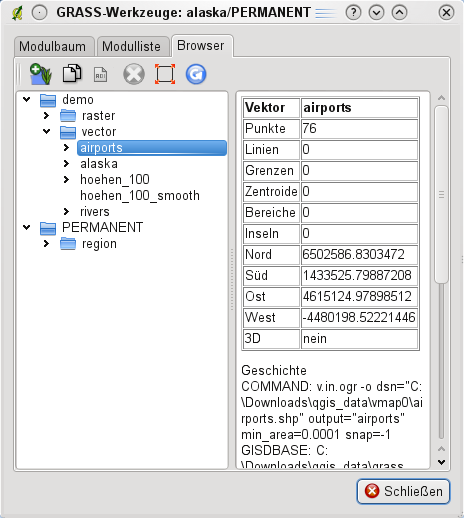
\includegraphics[clip=true,width=10cm]{grass_mapset_browser}
 \end{center}
\end{figure}

%The toolbar inside the \tab{Browser} tab offers following tools to manage the selected \filename{LOCATION}:
La barre d'outils de l'onglet \tab{Parcourir} donne accès à des outils de gestion du \filename{SECTEUR} sélectionné :

\begin{itemize}
%\item \toolboxtwo{grass_add_map}{Add selected map to canvas}
%\item \toolboxtwo{grass_copy_map}{Copy selected map}
%\item \toolboxtwo{grass_rename_map}{Rename selected map}
%\item \toolboxtwo{grass_delete_map}{Delete selected map}
%\item \toolboxtwo{grass_set_region}{Set current region to selected map}
%\item \toolboxtwo{grass_refresh}{Refresh browser window}
\item \toolboxtwo{grass_add_map}{Ajoute la carte sélectionnée à la carte QGIS}
\item \toolboxtwo{grass_copy_map}{Copie la carte sélectionnée}
\item \toolboxtwo{grass_rename_map}{Renomme la carte sélectionnée}
\item \toolboxtwo{grass_delete_map}{Efface la carte sélectionnée}
\item \toolboxtwo{grass_set_region}{Région courante réglée sur la carte choisie}
\item \toolboxtwo{grass_refresh}{Rafraîchir}

\end{itemize}

%The \toolboxtwo{grass_rename_map}{Rename selected map} and \toolboxtwo{grass_delete_map}{Delete selected map} only work with maps inside 
%your currently selected \filename{MAPSET}. All other tools also work with raster and vector layers in another \filename{MAPSET}.
Les commandes \toolboxtwo{grass_rename_map}{Renomme la carte sélectionnée} et \toolboxtwo{grass_delete_map}{Efface la carte sélectionnée} ne fonctionnent qu'avec les cartes présente dans votre \filename{Jeu de Données} sélectionné. Tous les autres outils fonctionnent aussi avec les autres \filename{Jeux de Données}.

%\subsubsection{Customizing the GRASS Toolbox} \index{GRASS!toolbox!customize}
\subsubsection{Personnaliser la boîte à outils GRASS} \index{GRASS!boîte à outils!personnaliser}
\label{sec:toolbox-customizing}

%Nearly all GRASS modules can be added to the GRASS toolbox. A XML interface is provided to parse the pretty simple XML files which configures 
%the modules appearance and parameters inside the toolbox.
Pratiquement tous les modules GRASS peuvent être ajoutés à la boîte à outils. Une interface XML est fournie pour analyser les fichiers XML 
très simple qui configurent l'apparence et les paramètres des modules dans la boîte à outils.

%A sample XML file for generating the module \usertext{v.buffer} (v.buffer.qgm) looks like this:
Un exemple de fichier XML pour le module \usertext{v.buffer} (v.buffer.qgm) est donné ci-dessous :
\begin{verbatim}
<?xml version="1.0" encoding="UTF-8"?>
<!DOCTYPE qgisgrassmodule SYSTEM "http://mrcc.com/qgisgrassmodule.dtd">

<qgisgrassmodule label="Vector buffer" module="v.buffer">
        <option key="input" typeoption="type" layeroption="layer" />
        <option key="buffer"/>
        <option key="output" />
</qgisgrassmodule>
\end{verbatim}

%The parser reads this definition and creates a new tab inside the toolbox when you select the module. A more detailed description for adding new  modules, changing the modules group, etc. can be found on the QGIS wiki at \\\url{http://wiki.qgis.org/qgiswiki/Adding\_New\_Tools\_to\_the\_GRASS\_Toolbox}.
L'analyseur lit cette définition et crée un nouvel onglet à l'intérieur de la boîte à outils lorsque vous sélectionnez le module. Une description plus détaillée pour ajouter des modules, changer le groupe des modules, etc. est disponible sur le wiki QGIS à l'adresse \\\url{http://wiki.qgis.org/qgiswiki/Adding\_New\_Tools\_to\_the\_GRASS\_Toolbox}.